\chapter{Génomique comparée des procaryotes}
\label{chap:comp}

L'analyse comparée des génomes regroupe une grande diversité d'analyses et de thématiques. On peut diviser ces analyses en 3 grands domaines : l'analyse des séquences, l'analyse des structures et l'analyse fonctionnelle.  Avec la croissance exponentielle du nombre de génomes disponibles dans les banques (cf. \autoref{sec:db}), et des informations de structures et d'annotations liées, il est essentiel de comparer les nouvelles séquences à celles déjà connues. Cette comparaison permettra de déduire, entre autres, les fonctions qu'elles contiennent et leur lien évolutif. 

Dans cette partie, j'aborderai les concepts informatiques et les algorithmes utilisés dans les méthodes de génomique comparée. Je reviendrai aussi sur les notions présentées précédemment et comment elles sont appliquées dans les outils. Pour terminer, nous présenterons un type d'analyse de génomique comparée qui est largement présent dans mon travail de thèse, l'analyse de systèmes biologiques.

\section{Analyse comparative des génomes : méthodes et applications}
\label{sec:comp_gen}

Pour comparer les séquences, on mesure leur similarité. Si la similarité des séquences est significativement élevée, alors on peut faire l'hypothèse que les séquences sont homologues\footnote{\textit{N.B} : L'homologie est une conclusion qualitative de l'observation quantitative de la similarité. On considère qu'une similarité de 30 \% permet de dire que 2 séquence sont homologues.}. Ce principe de base simple se révèle être un problème non trivial étant donné l'ensemble des mécanismes gouvernant l'évolution des génomes procaryotes. Pour comparer les génomes sur la similarité des séquences, on peut utiliser les séquences nucléotidiques, mais aussi en fonction du contexte, les séquences d'ARN ou de protéines. Pour l'ADN et l'ARN, la similarité va se confondre avec la notion d'identité, par contre pour les séquences d'acides aminés ces termes n'ont pas le même sens. Lorsqu'on mesure l'identité de séquences entre 2 protéines, on mesure le pourcentage de résidus identiques entre 2 séquences alignées. Pour la similarité, si les 2 acides aminés ont les mêmes propriétés physico-chimiques, ils seront considérés comme similaires. La mesure d'identité entre 2 séquences d'acides aminés sera toujours inférieure ou égale à celle de sa similarité.

Dans la suite, je ferai une revue (non exhaustive) des méthodes et des outils de génomique comparée. L'évolution de ces outils est intimement liée à l'évolution des techniques de séquençage, augmentant le volume de génomes disponibles, et à l'amélioration des technologies informatiques, augmentant les ressources disponibles et leur utilisation. 

\subsection{Alignement des séquences}

L'alignement des séquences peut être : pair ou multiple. Dans les deux cas, l'objectif est de trouver l'alignement qui maximise la correspondance entre les résidus. Pour cela, les séquences ne seront pas majoritairement pas alignées entre leur début et leur fin, elles seront décalées. Il existe alors 2 stratégies pour l'alignement : global et local. Dans un alignement global, on fait l'hypothèse que les séquences sont relativement similaires et donc on peut les aligner sur toute leur longueur.% Cette stratégie est bien adaptée pour les séquences proches
Pour un alignement local, on ne fait pas cette hypothèse et on cherche les régions dans la séquence qui ont le plus de similarité sans prendre en compte le reste de la séquence. Les algorithmes et outils que je vais présenter ensuite peuvent généralement s'appliquer au 2 types de stratégies, qu'on choisit en fonction du contexte.

\paragraph{Alignement par paire}

Dès les années 1960, on commence à voir des développements autour de l'idée de comparer 2 séquences (protéiques), mais c'est en 1970 que Needleman et Wunch présentent leur algorithme fondateur des approches de génomique comparée \cite{needleman_general_1970}. Leur algorithme d'alignement global repose sur la construction d'une matrice de similarité, représentant en ligne une séquence et en colonne la seconde, et inclut une pénalité de trou (\textit{gap} en anglais). Ainsi, il est possible de déterminer l'alignement optimal en considérant tous les \textit{gap} sans énumérer toutes les possibilités. Cet algorithme sera revu par Smith et Waterman qui, en 1981, proposent un nouvel algorithme, cette fois pour l'alignement local \cite{smith_identification_1981}. Ces 2 algorithmes ont l'intérêt de donner un résultat de comparaison exacte et sont d'ailleurs encore utilisés aujourd'hui. Toutefois, avec l'augmentation du volume de séquences, la comparaison de paire de séquences utilisant des algorithmes exhaustifs\footnote{Un algorithme exhaustif recherche toutes les solutions possibles pour trouver celle qui exacte ou optimale} pose un problème de complexité quadratique\footnote{La complexité d'un algorithme mesure la consommation de ressources (temps ou espace) nécessaire pour son exécution.}.

En 1985 et 1988, sont publiés les programmes FASTP et FASTA\footnote{Le format de données de l'outil FASTA est aujourd'hui utilisé comme format standard pour écrire les séquences. Les fichiers ont donc pris l'extension .fasta.} \cite{lipman_rapid_1985,pearson_improved_1988} qui marqueront un tournant en utilisant une approche heuristique\footnote{Un algorithme heuristique fournit un résultat rapidement, mais qui n'est pas nécessairement optimal ou exact.}. Le principe est de chercher quelles séquences peuvent être similaires en comparant des mots de tailles k (\textit{k-mer}), pour ensuite ne faire l'alignement exact que sur ce sous-ensemble de séquences. Dans la suite, en 1990, apparait le programme BLAST \cite{altschul_basic_1990}, qui utilise aussi cette approche heuristique et qui sera intégré comme outil dans les bases de données du NCBI, faisant sa renommée.  

Toujours lié à l'augmentation du volume de données, les outils utilisant ces approches heuristiques vont se perfectionner pour permettre l'alignement de paire de séquence de manière rapide et efficace, comme LAST \cite{kielbasa_adaptive_2011} ou DIAMOND \cite{buchfink_fast_2015}. 

\paragraph{Alignement multiple}
\label{paragraph:MSA}

L'alignement multiple des séquences (MSA pour \textit{Multiple Sequence Alignment} en anglais) vise à aligner plusieurs séquences simultanément. C'est une extension de l'alignement en paire. Ces alignements ont l'intérêt de révéler des régions conservées et ainsi d'identifier des relations évolutives, par contre la complexité est accrue et il est donc nécessaire d'introduire des algorithmes plus puissants.

Les premiers algorithmes étaient des algorithmes exhaustifs \cite{stoye_multiple_1998}, et tout comme pour l'alignement de paire de séquences, rapidement des algorithmes heuristiques ont été publiés. En 1988, Higgins et Sharp publient CLUSTAL \cite{higgins_clustal_1988}, une méthode d'alignement progressive pour obtenir un alignement multiple. Elle construit l’alignement en assemblant progressivement les séquences selon une hiérarchie basée sur une matrice de distance ou un arbre guide. D'autres méthodes adopterons cette approche, comme MUSCLE \cite{edgar_muscle_2004} mais ce dernier apporte un côté itératif. Ces méthodes sont rapides, mais peuvent être sensibles aux erreurs accumulées dans les étapes initiales.

D'autres méthodes, que je décrirai ensuite, s'appuient sur des éléments de statistique ou sur des algorithmes de graphes pour être plus efficaces. Il est à noter que toutes ces méthodes ont leur avantage et leurs inconvénients, qui doivent être évalués en fonction du contexte.

\subsection{Utilisation des graphes en génomique comparée}

Les graphes sont largement utilisés en bioinformatique \cite{pavlopoulos_using_2011} et ce dans des domaines très divers : interactions protéine-protéine, expression des gènes, modélisation du métabolisme\dots 

Dans mes travaux de thèse, je me suis largement appuyé sur les méthodes de graphes, il est donc essentiel de revenir sur la terminologie et les concepts liés à la théorie des graphes. Nous utiliserons le graphe de la \autoref{fig:graphe_theorie} pour illustrer les principes suivants.

\begin{figure}[htbp]
    \centering
    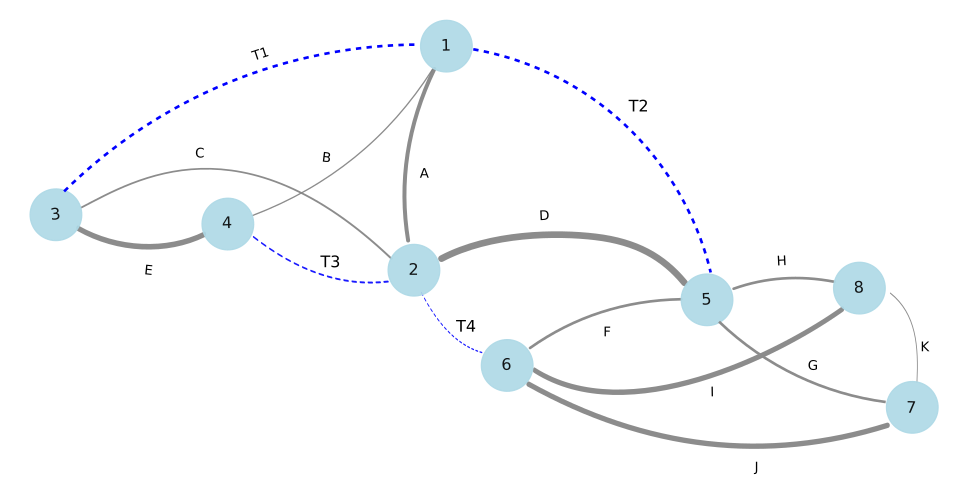
\includegraphics[width=\linewidth]{images/graphe_theorie_non_orienter.png}
    \caption[Exemple de graphe]{\textbf{Exemple de graphe.} Les n\oe uds sont représentés par des cercles et étiquetés par des numéros. Les arêtes, illustrées par des lignes pleines grises et étiquetées par une lettre, définissent les connexions entre les n\oe uds. L’épaisseur des arêtes est proportionnelle à leur poids, indiquant ainsi la valeur associée à chaque connexion. Les arêtes en pointillés bleus représentent les fermetures transitives du graphe, elles sont également étiquetées et pondérées pour expliciter les relations indirectes créées par la transitivité.}
    \label{fig:graphe_theorie}
\end{figure}

\subsubsection{Définitions et concepts}

Un graphe est constitué d'un ensemble de \textbf{n\oe uds} (cercles) reliés par un ensemble d'\textbf{arêtes} (segments gris). Mathématiquement, tous les graphes ne possèdent pas les mêmes propriétés et donc les théorèmes associés changent. Dans la suite, nous utiliserons les symboles mathématiques suivants :
\begin{itemize}
    \item $V$ : ensemble de n\oe uds
    \item $E$ : ensemble d'arêtes
    \item $G(V, E)$ : un graphe composé d'un ensemble de n\oe uds $V$ et d'arête $E$
    \item $u$ et $v$ : 2 n\oe uds distincts dans le graphe
    \item $e_{(u,v)}$ : une arête reliant $u$ et $v$.
\end{itemize}

\paragraph{Orientation du graphe}

Un graphe peut être \textbf{orienté}, \textit{i.e.}, que les arêtes ont une direction. Dans ce cas, il peut exister une arête de $u$ vers $v$ ($e_{(u, v)}$) sans qu'il n'y ait nécessairement une arête $e_{(v, u)}$. Si le graphe est non orienté, si $e_{(u, v)}$ existe, $e_{(v, u)}$ également. Dans notre exemple, le graphe est non orienté.

\paragraph{graphe pondéré et étiqueté}

En bioinformatique, il est courant d'ajouter de l'information sur le graphe. Ces informations peuvent servir à modifier le graphe, le filtrer ou l'analyser, par exemple.

On peut ajouter un \textbf{poids} aux n\oe uds ($w_u$) et aux arêtes ($w_{(u,v)}$), le graphe est alors dit \textbf{pondéré}. Le poids est quantifiable et correspond généralement à un nombre. Dans notre exemple, chaque arête a une épaisseur correspondant à son poids. On peut alors filtrer le graphe pour ne conserver que les arêtes les plus épaisses.

D'autres informations peuvent être ajoutées aux n\oe uds et aux arêtes sous forme d'annotation. Dans ce cas, l'annotation peut être qualitative et on dira que le graphe est \textbf{étiqueté}\footnote{Dans la littérature bioinformatique, on retrouve aussi le terme "coloré", mais qui est utilisé à tort si on se réfère à la théorie des graphes.}. Dans le graphe exemple, les arêtes sont étiquetées par une lettre et les n\oe uds par un chiffre. Cet étiquetage peut notamment correspondre à un identifiant.

\paragraph{Voisinage et chemin dans le graphe}

Dans cette thèse, nous parlerons de n\oe uds \textbf{voisins}, \textit{i.e.}, des n\oe uds qui sont reliés par un ensemble d'arêtes ($E_{(u,v)}$), cet ensemble d'arêtes est appelé \textbf{chemin}. Lorsque $u$ et $v$ sont reliés par une seule arête (chemin de taille 1), on dit qu'ils sont dans un \textbf{voisinage direct}. Dans notre exemple, le n\oe ud 1 est un voisin direct des n\oe uds 2 et 4 et est voisin des n\oe uds 3 et 5 par un chemin de taille 2. Lorsque tous les n\oe uds sont voisins les uns des autres, on dit que le graphe est \textbf{connexe}.

\newpage
\paragraph{Transitivité}

La \textbf{transitivité} dans les graphes est une propriété qui s'applique aux relations entre les n\oe uds. Un graphe est dit \textbf{transitif} si, pour tous n\oe uds $u$, $v$ et $w$, l'existence des arêtes $e_{u,v}$ et $e_{v, w}$, implique qu'il existe $e_{u,w}$. En d'autres termes, si $u$ et $v$ sont reliés et que $v$ et $w$ aussi, alors $u$ et $w$ sont reliés. Dans un graphe orienté transitif, s'il existe $e_{u,v}$ et $e_{v, w}$, alors il existe $e_{u, w}$, mais pas obligatoirement $e_{w, u}$. Cette propriété est particulièrement importante dans les graphes orientés, où elle peut être utilisée pour modéliser des relations hiérarchiques ou des dépendances. 

Dans notre exemple, le graphe n'est pas transitif. Pour le rendre transitif, on ajoute des \textbf{fermetures transitives} entre les n\oe uds. Ces arêtes de transitivité (en pointillés bleus) permettent de compléter le graphe pour le rendre transitif, facilitant ainsi l'analyse des relations et des dépendances implicites entre les n\oe uds.

\paragraph{Sous-ensemble du graphe}

Lorsqu'on va analyser un graphe, on peut chercher à retrouver des structures d'intérêt. Pour commencer, on peut chercher à identifier un \textbf{sous-graphe}. Le sous-graphe est une fraction du graphe qui contient un sous-ensemble de n\oe uds de $G(V, E)$ et les arêtes reliant ces n\oe uds. 

Une autre structure est la \textbf{clique}, qui correspond à un sous-ensemble de n\oe uds tous connectés entre eux. La détection et l'analyse de cliques a de nombreuses applications en bioinformatique, notamment l'identification de groupes de gènes coexprimés. Dans notre exemple, les n\oe uds 5,6,7 et 8 représentent une clique. 

Pour terminer, une forme de sous-ensemble que j'ai largement utilisée, est la \textbf{composante connexe} qui correspond à un ensemble de n\oe uds tel que, quel que soit $u$, $v$, il existe un chemin  qui les relie\footnote{La clique est une composante connexe spéciale où tous les n\oe uds sont reliés par un chemin de taille 1.}.

\paragraph{Partitionnement du graphe}

\textbf{Partitionner} un graphe consiste à diviser les n\oe uds du graphe en groupes. Chacun de ces groupes est appelé une \textbf{partie} et l'ensemble des parties est appelé \textbf{partition}. En fonction de l'algorithme utilisé, la partition sera alors différente. Dans ce manuscrit, nous utiliserons cette notion de partition à  de nombreuses reprises.

\subsubsection{Application dans la comparaison des génomes}

L'utilisation des graphes pour la comparaison de génomes est de plus en plus courante. 

Une première application possible est d'améliorer les méthodes de MSA. Des outils comme MUSCLE ou MAFFT \cite{katoh_mafft_2013} utilisent des arbres guides pour améliorer les performances de l'alignement. Ces arbres sont des graphes particuliers, où les séquences sont des n\oe uds et les relations de similarité sont des arêtes.

\newpage
Une seconde utilisation des graphes concerne l'étude des SNPs, indels et SVs. Ces graphes, appelés graphes de variants, représentent d'une manière flexible les différences entre les génomes. Chaque n\oe ud représente une séquence ou un k-mer, les arêtes vont représenter la colocalisation dans le génome. Ainsi, chaque chemin permet de reconstruire un génome, tout en ayant toutes les variations génétiques. Des outils comme VG toolkit \cite{garrison_variation_2018} et Minigraph \cite{li_design_2020}, permettent notamment d'améliorer l'alignement des lectures en sortie de séquençage, mais aussi d'enrichir la représentation des génomes procaryotes présentant une forte diversité.

Une autre application proche des graphes de variants est celle des graphes de réarrangements. Dans ces graphes, les n\oe uds représentent des synténies conservées, les arêtes vont relier ces synténies en fonction de l'ordre et de l'orientation dans les génomes. L'outil Sibelia \cite{minkin_sibelia_2013} est un outil d'alignement et d'analyse des réarrangements de génomes procaryotes. Il permet  d'étudier les différences évolutives et de reconstruire l'histoire des réplicons.



\subsection{Modèle statistique pour l'alignement des séquences}

Pour comparer de plus en plus de génomes, de nouvelles méthodes vont s'appuyer sur la modélisation statistique des séquences pour améliorer les performances de l'alignement et aligner de grands jeux de données. Chaque modèle représentera un ensemble de séquences et établit une fréquence ou probabilité d'un résidu pour chaque position. Ce modèle peut être assimilé à une séquence "consensus" du groupe.

\subsubsection{Partitionnement des séquences par similarité. }
\label{sec:clustering}

Les méthodes de partitionnement, ou \textit{clustering} en anglais, reposent sur les méthodes d'alignement pour déterminer la similarité des séquences, et les graphes pour représenter les liens de similarité entre chaque séquence. 

De manière générale, on va regrouper les séquences en groupes d'homologues en utilisant un seuil de similarité plus ou moins élevé. Les outils sont régulièrement présentés en utilisant la séquence protéique plutôt que nucléique pour calculer la similarité. Ce choix permet de réduire la complexité tout en étant plus précis sur l'évaluation de la similarité fonctionnelle et structurelle, mais aussi d'identifier des homologies plus lointaines. Dans ce cas, il faudra faire attention à la nuance entre similarité et identité. Ce qui va varier entre les méthodes, c'est l'algorithme de partitionnement utilisé. Le \autoref{tab:clustering} présente un aperçu des méthodes et des outils existants.  

\begin{table}[htbp]
    \footnotesize
    \centering
    \begin{tabular}{|p{0.2\textwidth}|p{0.25\textwidth}|p{0.25\textwidth}|p{0.25\textwidth}|}
\hline
\textbf{Outil} & \textbf{Description} & \textbf{Avantages} & \textbf{Inconvénients} \\
\hline
COGs \cite{tatusov_genomic_1997} & Classification basée sur l'évolution. Les clusters obtenus sont des groupes de protéines orthologues & Base de données bien documentées et largement utilisée & Méthode statique, mise à jour peu fréquente. \\
\hline
CD-HIT \cite{li_clustering_2001} & Clustering rapide basé sur la longueur des séquences, en ordonnant les protéines de la plus longue à la plus courte & Très rapide et efficace pour réduire la redondance & Sensibilité limitée pour les faibles identités de séquence \\
\hline
InParanoid \cite{remm_automatic_2001} & Détection des orthologues et paralogues en comparant deux génomes & Fiable pour détecter des orthologues proches, distingue bien orthologues et paralogues & Moins adapté aux comparaisons multi-génomes \\
\hline
OrthoMCL \cite{li_orthomcl_2003} & Identification des orthologues et paralogues récents via une approche basée sur les graphes & Bonne précision, adaptable à divers organismes & Consommation élevée en ressources pour les grands ensembles de données \\
\hline
UCLUST \cite{edgar_search_2010} & Alignement et clustering rapide des séquences protéiques & Très rapide, faible consommation mémoire & Moins précis que BLAST pour certaines comparaisons \\
\hline
Proteinortho \cite{lechner_proteinortho_2011} & Détection rapide d'orthologues à grande échelle & Évolutif et performant pour l'analyse de nombreux génomes & Moins détaillé sur les relations fonctionnelles des protéines \\
\hline
BUSCO \cite{simao_busco_2015} & Évaluation de la complétude des génomes en utilisant des ensembles de gènes conservés & Référence fiable pour les génomes récemment séquencés & Ne permet pas une recherche extensive d'orthologues \\
\hline
OMA \cite{altenhoff_oma_2019} & Méthode évolutive d'identification des orthologues & Haute précision sur les génomes bien annotés & Temps de calcul élevé pour les grands jeux de données \\
\hline
SwiftOrtho \cite{hu_swiftortho_2019} & Similaire à OrthoMCL, utilisant des k-mers longs pour améliorer la rapidité & Très rapide et nécessite peu de ressources & Peut être moins précis pour des génomes très divergents \\
\hline
SonicParanoid \cite{cosentino_sonicparanoid_2019} & Extension de InParanoid pour la détection rapide d'orthologues & Améliore la vitesse et réduit les besoins en ressources & Moins précis pour des génomes très distants évolutivement \\
\hline
OrthoFinder \cite{emms_orthofinder_2019} & Détection des orthologues basée sur une approche évolutive & Haute précision grâce à l'utilisation de scores de similarité normalisés & Temps de calcul élevé pour les grands ensembles de données \\
\hline
OrthoPhy \cite{watanabe_orthophy_2023} & Intègre les informations taxonomiques dans l'identification des orthologues & Minimise les erreurs de prédiction et améliore la fiabilité & Exige davantage de ressources et est plus lent sur de grandes bases de données \\
\hline
\end{tabular}
\caption[Outils de clustering des séquences]{\textbf{Présentation des principaux  outils de clustering de séquences avec leurs descriptions, avantages et inconvénients.}}
\label{tab:clustering}
\end{table}

\newpage
\subsubsection{MMSeqs2}

Un outil largement utilisé pour l'alignement et le \textit{clustering} de grand jeu de données est l'outil MMSeqs2 \cite{steinegger_mmseqs2_2017}. L'objectif de MMSeqs2 est de partitionner les séquences en groupes d'homologues, de manière rapide et efficace. MMSeqs2 s'appuie sur les technologies informatiques, tant matérielles que logicielles, pour optimiser les ressources utilisées, et sur un nouvel algorithme de recherche de k-mer similaire. 

MMSeqs2 ne va pas faire des comparaisons exactes de k-mers, mais il va chercher des k-mers similaires. Cette différence permet de comparer les k-mers plus rapidement tout en utilisant des k-mers de plus grandes tailles, améliorant sa sensibilité\footnote{La sensibilité correspond au nombre de séquences qui sont alignées par rapport au nombre de séquences qui sont similaires.}. Comme présenté sur la \autoref{fig:mmseqs2}, les k-mers utilisés sont "espacés", ce qui permet un recouvrement plus important de la séquence et donc de réduire les alignements liés au hasard de k-mers successifs entre 2 séquences non homologues. S'appuyant sur cette caractéristique, les auteurs de MMSeqs2 vont supposer que si les séquences ont des k-mers similaires, séparé par le même nombre de résidus, alors la zone entre les k-mers à des chances de s'aligner, ce qui permet d'étendre les zones alignables (diagonale). Enfin, un score associé aux diagonales va être utilisé pour filtrer les séquences qui ont le plus de probabilités de s'aligner.

\begin{figure}[htbp]
    \centering
    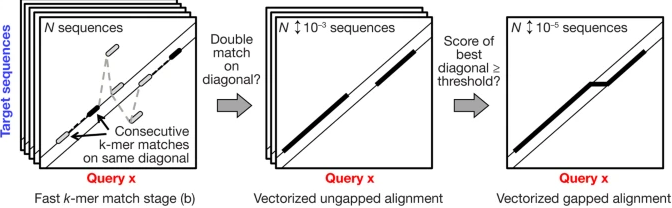
\includegraphics[width=\textwidth]{images/mmseqs2.png}
    \caption[Principe de l'alignement de MMSeqs2.]{\textbf{Principe de l'alignement de MMSeqs2.}  Extrait de \cite{steinegger_mmseqs2_2017}}
    \label{fig:mmseqs2}
\end{figure}

Une fois l'étape d'alignement terminée, MMSeqs2 intègre plusieurs algorithmes pour partitionner les séquences. Dans chacun de ces algorithmes, chaque groupe de séquences similaires (partie) verra une des séquences (n\oe ud) utilisée comme référente. (\textit{i}) L'algorithme Set-cover (\autoref{fig:set-cover}) sélectionne le n\oe ud avec le plus d'arêtes comme référent et forme une partie avec tous les n\oe uds dans un voisinage direct, puis de manière itérative reproduit le schéma jusqu'à ce que tous les n\oe uds soient dans une partie. (\textit{ii}) L'algorithme \textit{Connected Component} (\autoref{fig:connected-componet}) fonctionne comme Set-cover, mais partitionne tous les n\oe uds pour lesquels il existe un chemin avec le n\oe ud référent. (\textit{iii})  l'algorithme \textit{CD-hit like} (\autoref{fig:cdhit}) prend pour référence le n\oe ud dont le poids (taille de la séquence) est le plus élevé, puis forme une partie avec tous les voisins directs. Ces algorithmes répondent chacun à des problématiques différentes que nous pourrons illustrer dans la suite.  

\begin{figure}[htbp]
    \centering
    \subfloat[Set-cover]{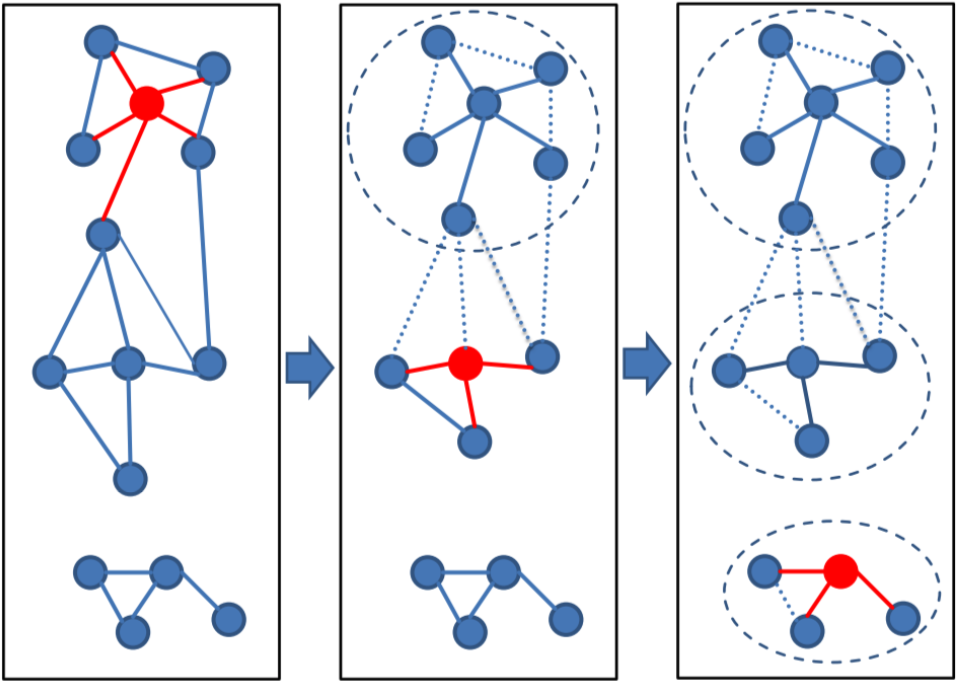
\includegraphics[width=.3\textwidth]{images/cluster-mode-setcover.png}
    \label{fig:set-cover}}
    \hfill
    \subfloat[Connected component]{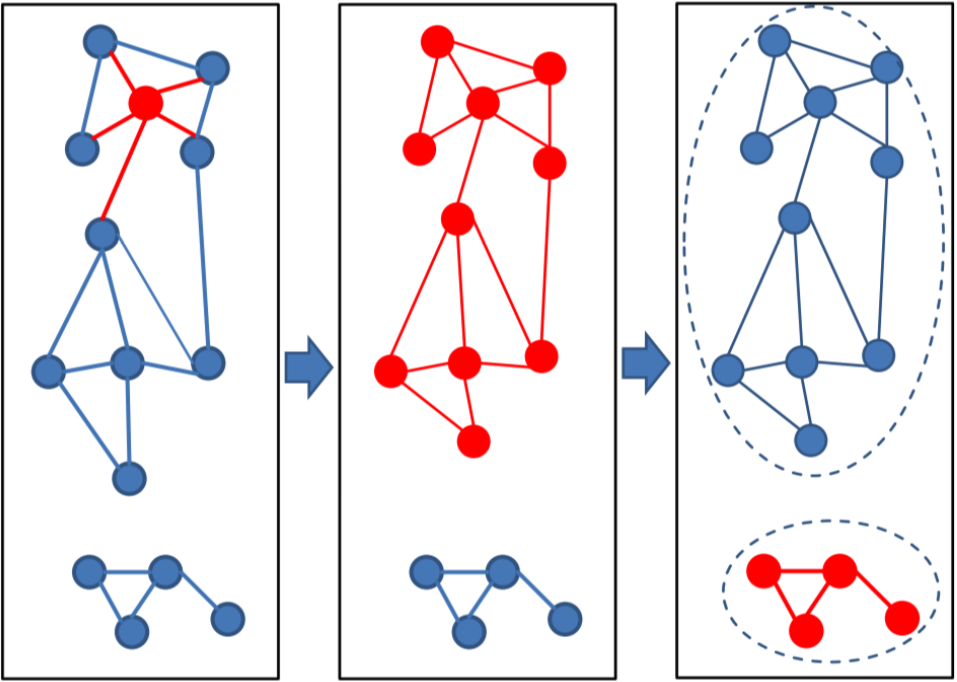
\includegraphics[width=.3\textwidth]{images/cluster-mode-connectedcomp.png}
    \label{fig:connected-componet}}
    \hfill
    \subfloat[CD-hit like]{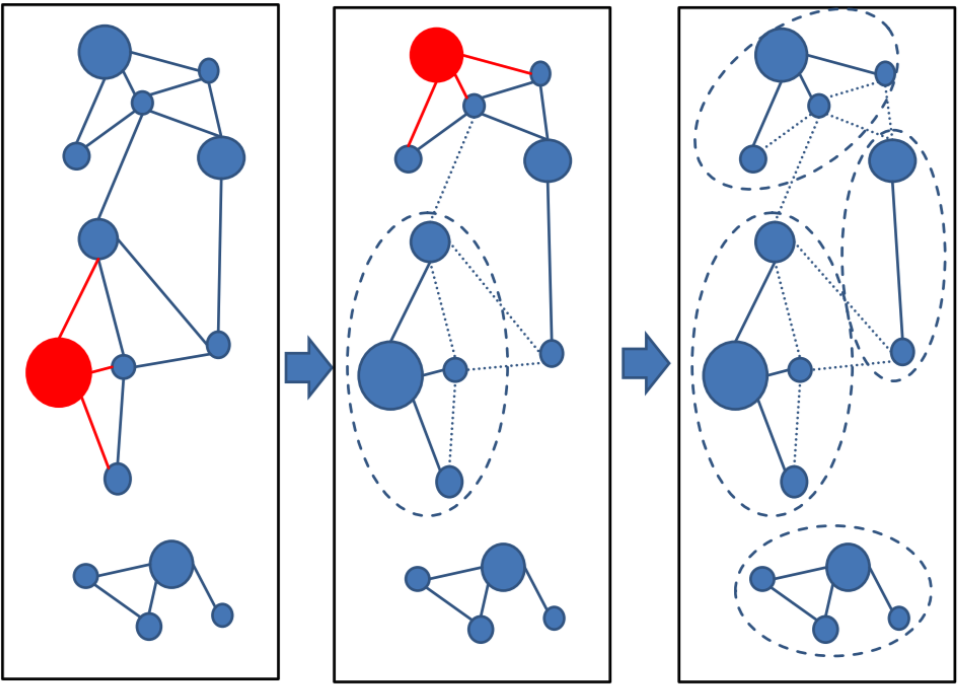
\includegraphics[width=.3\textwidth]{images/cluster-mode-greedyincremental.png}
    \label{fig:cdhit}}
    \caption[Algorithmes de clustering de MMSeqs2]{\textbf{Les algorithmes de clustering de MMSeqs2.}}
    \label{fig:mmclust}
\end{figure}

\newpage

Depuis 2018, MMSeqs2 intègre une nouvelle méthode appelée Linclust \cite{steinegger_clustering_2018}. Celle-ci vise à proposer un clustering dont la durée évolue linéairement avec le nombre de séquences. Pour ce faire, les séquences ne sont pas alignées entre elles. Dans un graphe, chaque séquence forme un n\oe ud et est représentée par des k-mers, eux-mêmes répartis en groupes. La séquence la plus longue de chaque groupe est comparée à toutes les autres. Si l'alignement dépasse un seuil prédéfini, une arête de similarité est établie entre les séquences. Ensuite, un algorithme de partitionnement est appliqué au graphe résultant pour obtenir le partitionnement final. Cette optimisation permet de partitionner rapidement de grands jeux de données.

\subsubsection{Modélisation des séquences similaires : matrices de position, profils et chaînes de Markov}

Une fois les séquences regroupées par similarité, il est possible de créer un modèle statistique représentant les séquences, sous forme de "séquence" consensus. L'idée générale de ces modèles va être, pour chaque position de la séquence consensus, d'associer pour chaque type de résidus une fréquence ou probabilité d'apparition, basée sur un alignement multiple des séquences.

Les premiers modèles statistiques correspondaient à des matrices de score à position spécifique (PSSM, position-specific scoring matrices), représentant la probabilité du résidu à une position donnée. Ainsi la matrice obtenue reflète pour un score positif une correspondance de résidus similaires parmi les séquences, ou pour un score négatif un résidu non conservé. Ces matrices ont été utilisées dans des outils comme CLUSTAL \cite{higgins_clustal_1988} ou MATCH$^{TM}$ \cite{kel_matchtm_2003} pour la recherche de facteur de transcription dans les séquences d'ADN, ou encore dans l'algorithme ESAsearch \cite{beckstette_fast_2006} pour rechercher des séquences dans les PSSMs. Ces outils vont également amener une variante aux PSSMs qui comble un défaut de ces dernières. En effet, le score dépend du nombre et de la divergence des séquences utilisées dans le MSA. Si la matrice est constituée de peu de séquences ou si des séquences proches sont surreprésentées, alors le score sera biaisé. C'est pourquoi un poids est appliqué pour réduire l'impact des séquences proches et augmenter celui des séquences divergentes. 

Pour construire une PSSM, les MSA doivent être continus (sans \textit{gap}), ce qui est rarement le cas. Une nouvelle forme de PSSM, appelée profil, va prendre en compte les \textit{gap} en appliquant des pénalités. Un profil est donc une PSSM intégrant les possibles indels sous forme de pénalités\footnote{Dans la littérature, les PSSM sont souvent également appelées profils.}. Les profils sont utilisés, notamment dans le contexte des bases de données, pour rechercher des séquences homologues à un groupe de séquences sans aligner chacune des séquences du groupe. PSI-BLAST \cite{altschul_gapped_1997}, développé par les auteurs de BLAST, permet de construire des profils et de rechercher des séquences contre un profil. Bien que PSI-BLAST soit reconnu pour sa haute précision, il demeure sensible aux erreurs d'assignation initiales, lesquelles peuvent introduire des biais dans les profils générés et impacter la fiabilité des cycles et des itérations suivants.

Une dernière forme de modèle s'appuie sur les chaînes de Markov cachées (\textit{Hidden Markov Model} en anglais, HMMs). Une chaîne de Markov décrit la probabilité de transition vers un état en fonction des états précédents. Dans nos modèles, cela correspondrait à calculer la probabilité d'un résidu (état) à une position donnée en fonction des résidus des positions précédentes. Une chaîne de Markov cachée inclut, en plus, l'existence de facteurs non observables sur la probabilité de transition. Dans nos modèles, ces facteurs cachés peuvent être les \textit{gaps} qui ne correspondent à aucun résidu (état) mais influencent la probabilité de transition (\autoref{fig:HMM_ex}). On peut alors obtenir une probabilité pour chaque résidu à chaque position. 

\begin{figure}[htbp]
    \centering
    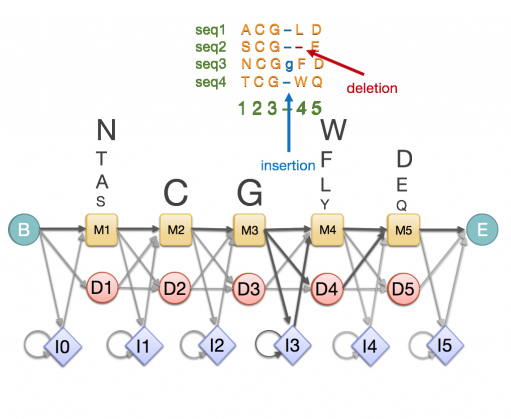
\includegraphics[width=0.5\linewidth]{images/HMM_ex.png}
    \caption[Exemple de modélisation HMM d'une séquence]{\textbf{Exemple de modélisation HMM d'une séquence.} Les cases jaunes représentent les états de correspondance (M), où la distribution de probabilité est déterminée par la fréquence des acides aminés à cette position. La rangée d'états en forme de losange correspond aux états d'insertion (I) et les états circulaires désignent les états de suppression (D). Ce modèle probabiliste permet d’estimer les fréquences observées des acides aminés à chaque position et de représenter les transitions entre eux, sur la base de l’occupation observée des positions dans un alignement de séquences multiples. Extrait de \url{https://www.ebi.ac.uk/training/online/courses/pfam-creating-protein-families/what-are-profile-hidden-markov-models-hmms/}}
    \label{fig:HMM_ex}
\end{figure}

Les modèles HMMs semblent donc tout indiqués pour représenter l'alignement des séquences similaires. Les HMMs, ont l'intérêt de pouvoir différencier les événements d'insertion des événements de délétion par rapport aux profils. Cet avantage les rend plus robustes que les profils. 

Un outil largement utilisé pour construire des HMMs et rechercher des séquences homologues contre une base de données HMMs est HMMER (\url{http://hmmer.org/}). Un autre outil, HH-suite \cite{steinegger_hh-suite3_2019}  intègre la possibilité de faire des comparaisons HMM/HMM. Ces outils, dans leurs versions récentes, ont été optimisés pour combler la complexité sous-jacente de l'utilisation de tels modèles. D'autres outils récents, comme ApHMM \cite{firtina_aphmm_2024} ou le package pyhmmer\cite{larralde_pyhmmer_2023}, proposent des améliorations techniques pour augmenter l'efficacité et la sensibilité des comparaisons aux HMMs, notamment pour ApHMM en s'appuyant sur les nouvelles technologies matérielles et logicielles, et en optimisant les calculs opérés par les algorithmes.

Les modèles HMMs sont couramment utilisés pour la recherche de séquences homologues dans les bases de données. Ils trouvent également des applications dans d'autres domaines, tels que la classification et l'annotation des protéines, ainsi que la prédiction de gènes et de promoteurs \cite{dimri_hidden_2024}.


\section{Analyse des Systèmes biologiques}
\label{sec:sys_bio}

La notion de système biologique est vaste et dépend du domaine et du contexte scientifique. Dans cette section, je vais définir les systèmes dans le cadre de la génomique comparée des procaryotes, en lien avec les processus métaboliques et cellulaires. J'aborderai l'état de l'art des méthodes bioinformatiques utilisées pour identifier les systèmes et je terminerai en décrivant un type particulier de système biologique : les systèmes de défense contre les phages, qui ont été au c\oe ur de mes développements méthodologiques.

\subsection{Définition et intérêt}

Un système biologique est constitué d’un ensemble de protéines interagissant pour réaliser un processus spécifique. Ces processus sont souvent régulés au sein d’opérons ou de groupes de gènes colocalisés. Les systèmes sont classés et nommés en fonction de leur rôle, comme ceux impliqués dans la conjugaison, regroupés sous l’appellation de \textbf{système conjugatif}.

La description et l'étude de ces systèmes est essentielle, car une fois caractérisé, ils permettent de comprendre les capacités métaboliques et les capacités d'adaptation des organismes \cite{alberts_cell_1998}. De plus, certains systèmes sont associés à des îlots génomiques, comme les systèmes de sécrétion de type III et VI associés aux îlots de pathogénicités\cite{pallen_bacterial_2007}. Leur identification dans les GIs est essentielle à la compréhension de l'adaptation et de la diversité des écosystèmes procaryotes. 

Les systèmes biologiques présentent une grande diversité de composition et d’organisation. Premièrement, certains gènes peuvent être facultatifs ou spécifiques à certaines niches écologiques. Par exemple, la réparation de l’ADN repose sur RecA, une protéine clé de la recombinaison homologue, mais peut aussi emprunter des voies alternatives, comme les systèmes RecBCD chez \textit{Escherichia coli} ou AddAB chez \textit{Helicobacter pylori}\footnote{Bactérie pathogène connue pour son rôle dans les infections gastriques et notamment dans les ulcères de l'estomac.} \cite{dillingham_recbcd_2008}. Un autre exemple concerne le système de sécrétion T2SS \cite{korotkov_type_2012}, présent dans un grand nombre de bactéries Gram-négatives pathogènes et non pathogènes. Il est composé de 4 protéines essentielles à son fonctionnement : gspD, gspE, gspF et gspG, mais peut aussi être trouvé dans les organismes avec des protéines supplémentaires facultatives : gspC, gspH, gspI, gspJ, gspK, gspL, gspM et gspN. Ces protéines facultatives peuvent être absentes dans certains taxons, comme chez les Chlamydiae pour T2SS \cite{abby_identification_2016}. Ensuite, des gènes peuvent avoir des homologues avec d’autres systèmes, parfois même très différents, rendant leur classification complexe. C’est notamment le cas du système de sécrétion de type VI, qui présente des similitudes structurelles avec les phages à queue contractile, suggérant une origine évolutive commune \cite{coulthurst_type_2013}. La dynamique évolutive des systèmes est également hétérogène. Certains composants sont fortement conservés, tandis que d'autres évoluent rapidement sous l'effet de pression de sélection. C'est le cas des systèmes de défense (cf. \autoref{sec:def}), tels que les systèmes CRISPR-Cas, dont la diversité des protéines Cas (permettent de découper l'ADN viral) reflète une adaptation continue contre les virus \cite{makarova_comparative_2013}. Cette variabilité complique alors l’identification des homologues par la seule comparaison de séquences.

\subsection{Méthodes de détection}

l'identification de systèmes repose sur la combinaison de la recherche des gènes et sur leur organisation en contexte. En s'appuyant sur ces propriétés, on peut alors identifier des systèmes connus ou proches chez les organismes.

Avant les années 2000, la recherche de systèmes biologiques était basée sur des approches phylogénétiques, en recherchant des homologues, ou par de l'annotation manuelle de régions d'intérêt comme les GIs \cite{buchrieser_high-pathogenicity_1998}. Des outils ont ensuite été développés pour détecter différents systèmes : les systèmes conjugatifs, les systèmes de sécrétion, les systèmes de défenses contre les phages (\autoref{sec:def}) et les systèmes métaboliques. Leur évolution a suivi une trajectoire marquée par des avancées méthodologiques, passant de simples bases de données statiques à des modèles probabilistes et des approches d’intelligence artificielle.

\paragraph{Systèmes de sécrétion et de conjugaison}

Les premiers outils pour la recherche de systèmes spécifiques, tels que les systèmes de sécrétion, annotaient fonctionnellement les génomes pour identifier les gènes codant des fonctions connues des systèmes. En 2008, l'outil ICEberg \cite{bi_iceberg_2012} a été développé pour identifier les ICEs (cf. \autoref{sec:evo_hz}) à partir d'une base de données de protéines annotées manuellement et d'un alignement avec BLASTp sur les génomes. Bien que régulièrement mise à jour \cite{wang_iceberg_2024}, cette base de données n'est pas adaptée à la détection des ICEs divergents, limitant ainsi son utilisation à des systèmes bien caractérisés. Pour pallier ces limites, l’outil ICEscreen \cite{lao_icescreen_2022} a été développé afin de détecter les ICEs et IMEs (\textit{Integrative and Mobilizable Elements}) des Firmicutes\footnote{Firmicutes, renommé en 2021 Bacillota est un phylum  }, qu'ils soient isolés ou intégrés dans des structures composites. Contrairement aux approches basées uniquement sur des bases de données de séquences connues, ICEscreen utilise des stratégies de détection basées sur des signatures génétiques et des relations de synténie, permettant ainsi d’identifier des éléments plus divergents ou moins bien caractérisés.

SecReT4 \cite{bi_secret4_2013} a proposé une base de données spécifique pour la détection des systèmes de type IV (T4SS). Bien que cette approche soit utile, elle est limitée par la nécessité de mises à jour régulières et une couverture incomplète des systèmes de sécrétion existants.

En 2014, MacSyFinder \cite{abby_macsyfinder_2014} a introduit une nouvelle approche en utilisant une base de données HMM pour annoter les gènes dans les génomes. Il a également introduit la notion de modèle de système pour décrire les composants du système et son organisation génomique (\autoref{fig:macsyfinder}). Par exemple, les modèles TXSScan \cite{abby_identification_2016} permettent de détecter les systèmes de sécrétion, tandis que TFFScan \cite{denise_diversification_2019} et CONJScan \cite{cury_integrative_2017} sont utilisés pour les filaments de type IV et les systèmes de conjugaison, respectivement.

\begin{figure}[htbp]
    \centering
    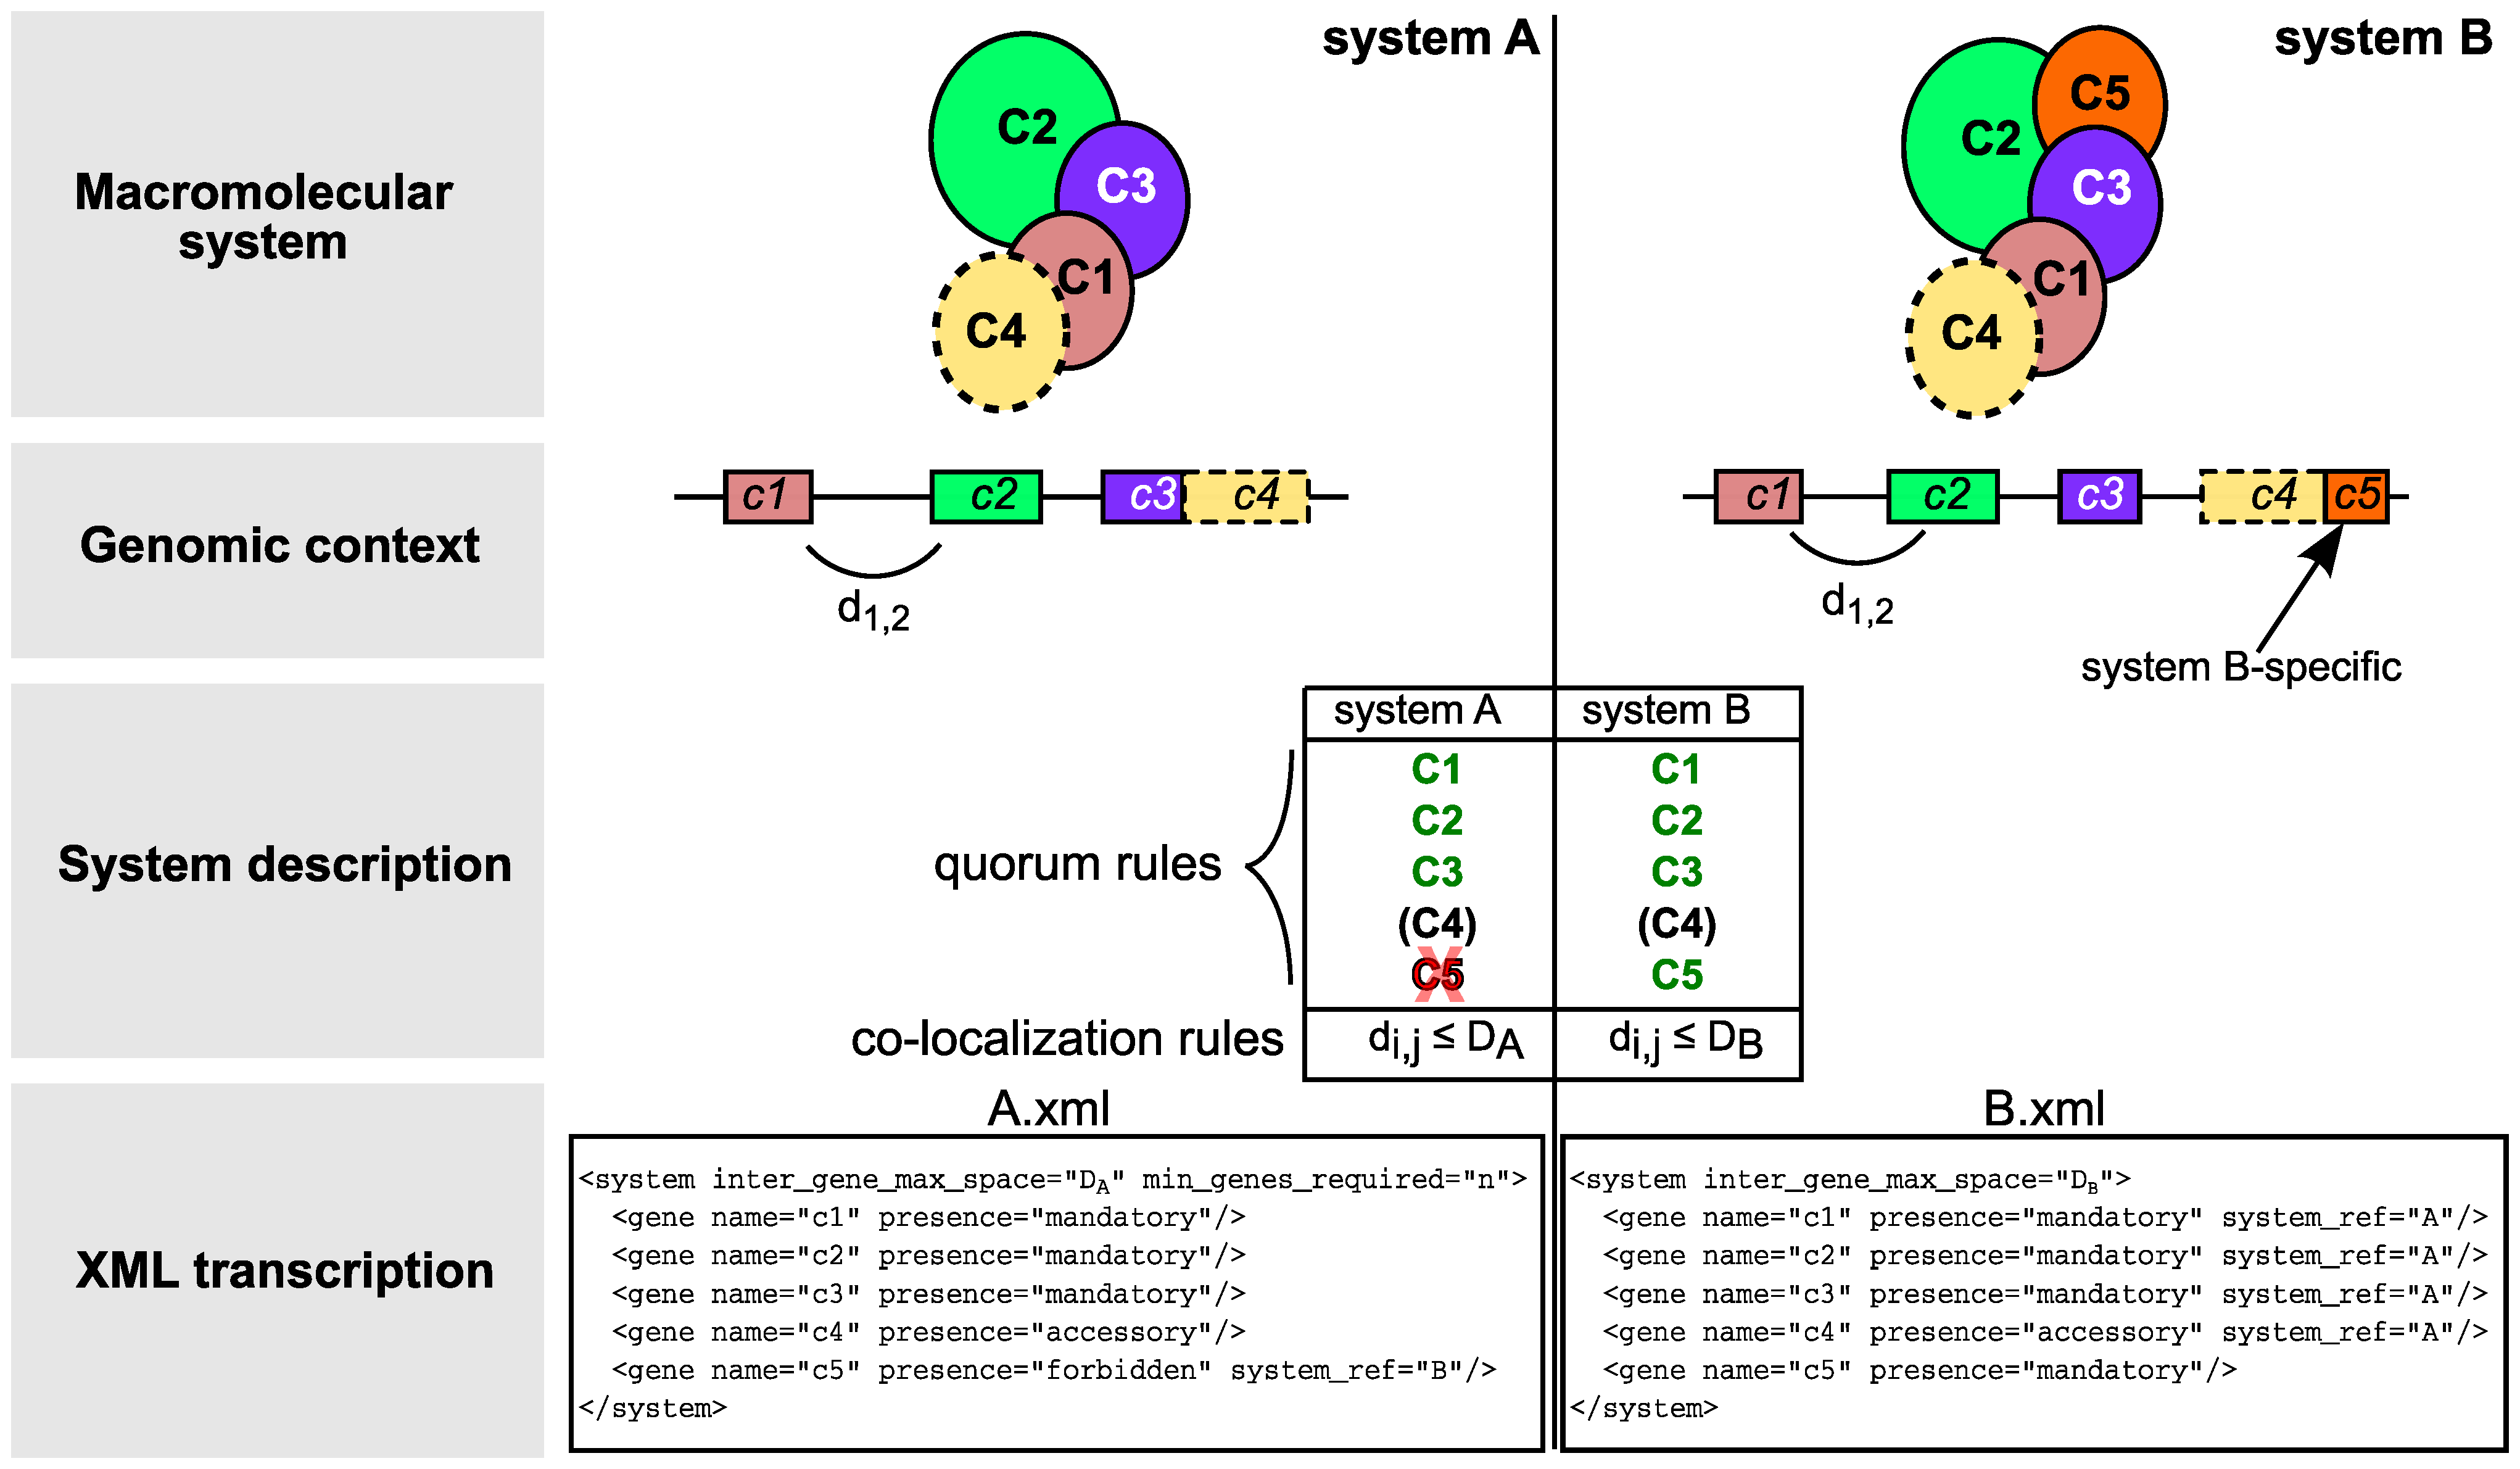
\includegraphics[width=\linewidth]{images/macsyfinder.png}
    \caption[Exemple de modélisation de systèmes dans MacSyFinder]{\textbf{Exemple de modélisation de systèmes dans MacSyFinder.} Extrait de \cite{abby_macsyfinder_2014}}
    \label{fig:macsyfinder}
\end{figure}

Plus récemment, T4SEpre \cite{wang_prediction_2014} et T4SEpp \cite{hu_t4sepp_2024} ont utilisé des modèles et des méthodes d'apprentissage automatique pour améliorer la sensibilité et la spécificité de la prédiction des systèmes T4SS.

\paragraph{Systèmes impliqués dans le métabolisme secondaire}

En 2011, antiSMASH \cite{medema_antismash_2011} a marqué une avancée majeure en automatisant l'identification des groupes de gènes colocalisés impliqués dans une voie de biosynthèse, appelés \textit{Biosynthetic Gene Clusters} (BGCs). Cette identification repose sur une vaste base de données de profils HMM, permettant la détection d'un large éventail de BGCs, notamment les NRPS (peptides non ribosomiques), les PKS (polykétides), les RIPP (\textit{Ribosomally Synthesized and Post-translationally Modified Peptides}) ainsi que d'autres métabolites secondaires.

Des méthodes récentes, telles que DeepBGC \cite{hannigan_deep_2019} et GECCO \cite{carroll_accurate_2021}, utilisent des modèles de \textit{deep learning} et des approches de traitement du langage naturel pour prédire les BGCs. Ces méthodes permettent une classification plus précise, bien qu'elles nécessitent une puissance de calcul importante et soient moins accessibles aux microbiologistes que les outils classiques.

\newpage

\subsection{Les systèmes de défense aux phages}
\label{sec:def}

Dans leur environnement naturel, les procaryotes sont fréquemment exposées à l’infection par des \textbf{phages}. Au fil de l’évolution, ces virus ont développé une remarquable diversité de mécanismes leur permettant d’infecter un éventail plus ou moins large d’espèces. Ces dernières années, l’intérêt pour les phages s’est considérablement accru, passant de 452 publications mentionnant le terme phage dans les MeSH Terms de PubMed en 2000 à 1250 en 2024. Cet engouement est notamment porté par la reconsidération de la \textbf{phagothérapie}\footnote{Utilisation des phages pour traiter certaines maladies en ciblant sélectivement les cellules.}, une approche permettant de combattre les infections bactériennes \cite{boniver_phage_2022}. Bien que cette stratégie thérapeutique ait été utilisée dès l’après Première Guerre mondiale, elle a progressivement été délaissée au profit des antibiotiques. Toutefois, la montée alarmante des souches bactériennes multirésistantes conduit aujourd’hui à réexaminer les phages comme une alternative thérapeutique.

Face à ces infections, les procaryotes ont, eux aussi, développé une vaste panoplie de mécanismes regroupés sous le terme \textbf{systèmes de défense contre les phages}. Cette compétition entraîne une course coévolutive, menant à une diversification continue des stratégies d’infection des phages et des systèmes de défense. Les microbiologistes s’intéressent de plus en plus à ces interactions complexes, non seulement pour leurs applications pratiques en génétique moléculaire, comme l’exploitation des enzymes de restriction, mais aussi pour leur potentiel dans le développement de la phagothérapie. La connaissance des mécanismes permettant à une souche de résister à une gamme spécifique de phages étant essentielle pour concevoir des traitements efficaces et adaptés.

\subsubsection{Phages : retour sur les virus de bactéries}
\label{sec:phage}
Les virus infectant les bactéries, connus sous le nom de bactériophages ou phages, ont été observés pour la première fois en 1915 et décrits officiellement par Félix d'Hérelle. Ces phages, dont la taille varie entre 20 et 200 nanomètres, présentent une grande diversité de formes. Leur matériel génétique peut être constitué d'ADN ou d'ARN, en simple ou double brin (\autoref{fig:phages}). Chaque phage possède un spectre d'hôtes spécifique, \textit{i.e}, qu'il ne peut infecter qu'un nombre restreint et défini d'espèces procaryotes.

\begin{figure}[htbp]
    \centering
    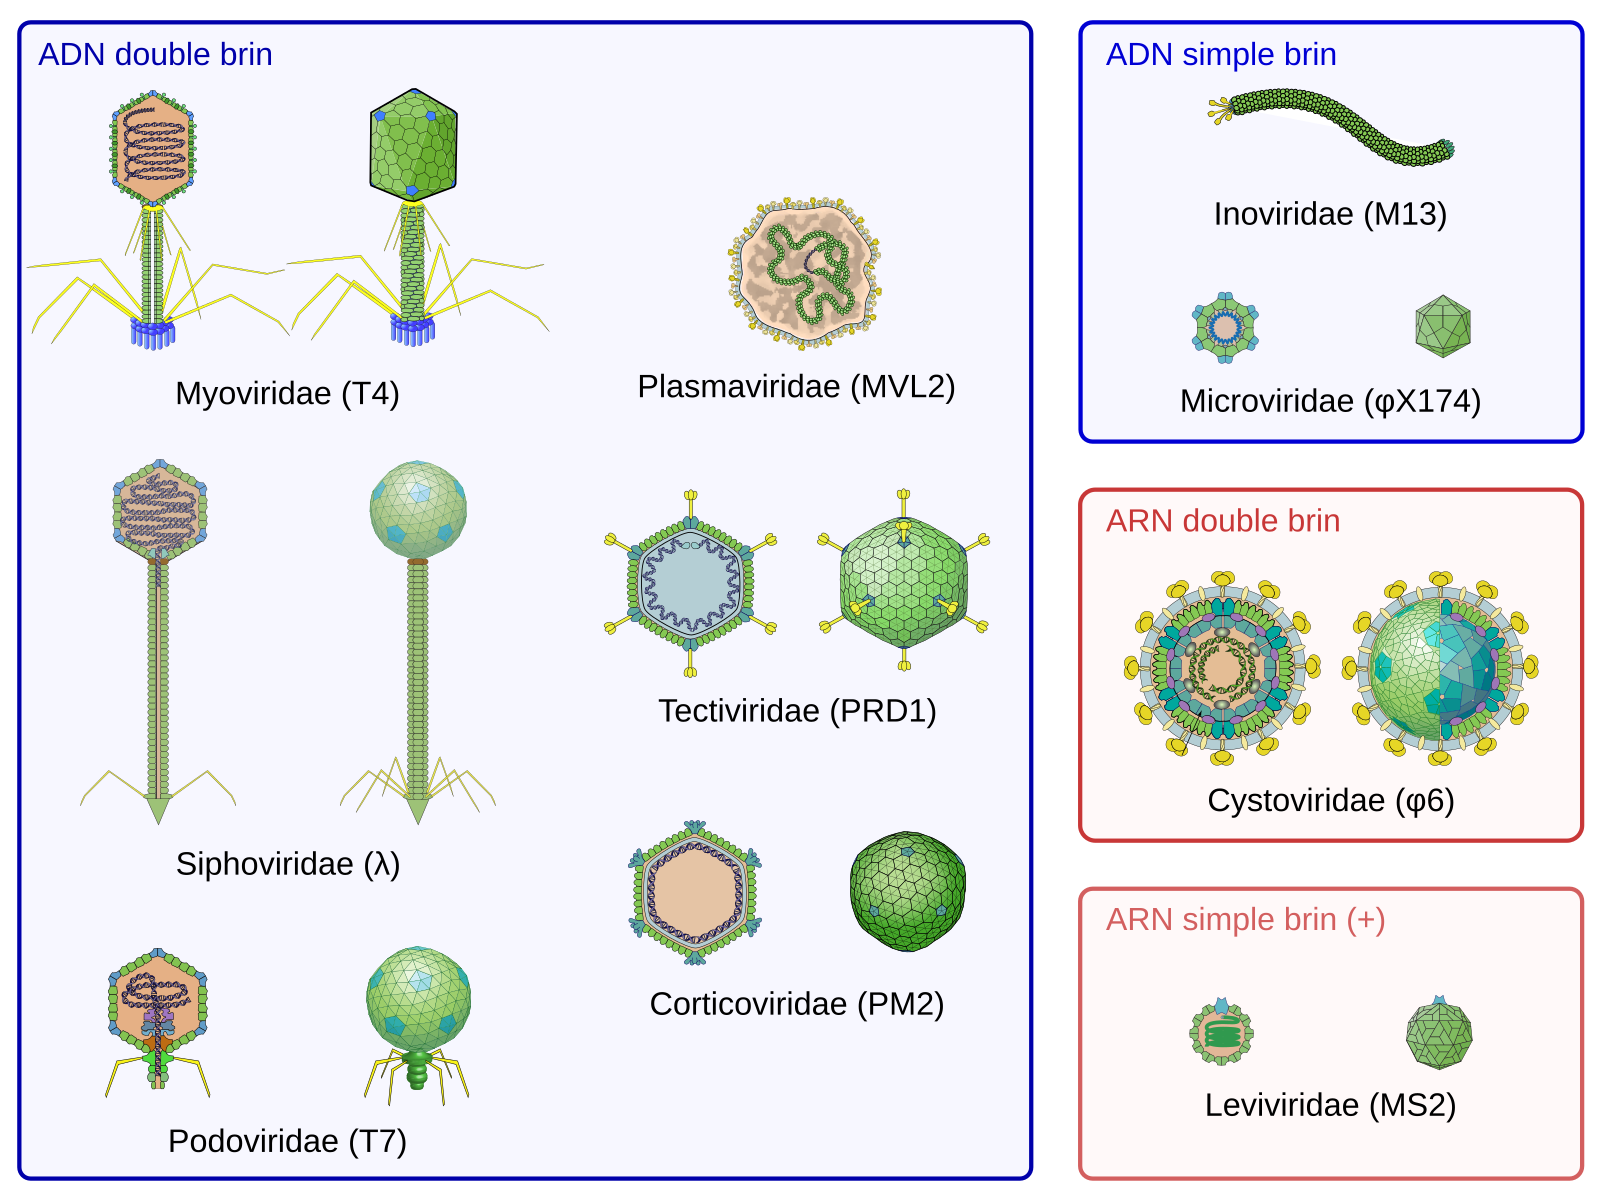
\includegraphics[width=0.75\linewidth]{images/phages.png}
    \caption[Diversité morphologique parmi les phages]{Diversité morphologique des phages. Auteur : Philippe Le Mercier - ViralZone SIB Swiss Institute of Bioinformatics}
    \label{fig:phages}
\end{figure}

Les phages ne sont pas capables de répliquer leur propre matériel génétique, c'est pourquoi ils infectent les cellules procaryotes, afin d'utiliser les systèmes de réplication de l'hôte. Une fois que le matériel a été répliqué (des milliers de fois), les nouveaux phages seront libérés dans l'environnement en lysant la cellule (ouverture de la paroi). Le cycle d'infection, réplication, libération existe sous 2 formes définissant 2 catégories de phages (\autoref{fig:cycle_phage}). Le cycle lytique, réalisé par les phages virulents, correspond à un cycle court où le phage détruit l'hôte à la fin de sa réplication. Le cycle lysogénique, opéré par les phages tempérés, réfère à un phage qui va rester dans la cellule pendant plusieurs cycles de réplication de l'hôte. Dans ce cas, le matériel génétique peut s'intégrer au chromosome de l'hôte et se répliquer avec lui, on parle de région prophagique, ou rester dans le cytoplasme sous forme d'épisome et se répliquer indépendamment comme un plasmide.

\begin{figure}
    \centering
    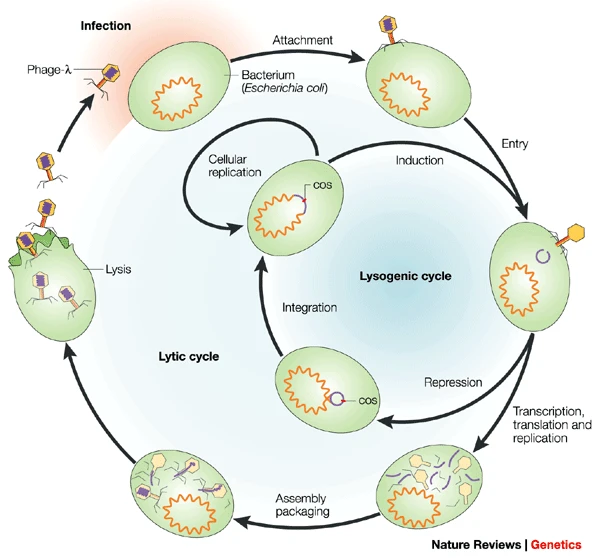
\includegraphics[width=0.75\linewidth]{images/cycle_phages.png}
    \caption[Cycle de vie des phages]{Cycle de vie des phages. Extrait de \cite{campbell_future_2003}}
    \label{fig:cycle_phage}
\end{figure}

\newpage
\subsubsection{Mécanismes de défense contre les phages}

Pour se défendre contre les phages, les procaryotes ont  développé un arsenal pour se protéger : les systèmes de défense contre les phages\footnote{que nous raccourcirons en systèmes de défense dans cette partie} \cite{makarova_comparative_2013}. Un système de défense correspond à un ensemble de protéines qui vont empêcher l'infection du phage et donc empêcher la destruction de la cellule. Ils peuvent agir de manière très diverse et à différent moment du cycle de vie du phage. 

%Dans la nature, il en existe une grande diversité et un organisme n'est capable d'en utiliser seulement une partie. 

Les premiers systèmes de défense ont été identifiés dans les années 50, il s'agit des systèmes de restriction-modification (RM) \cite{bertani_host_1953}. Ces systèmes sont composés de deux fonctions principales, généralement assurées par deux protéines distinctes : la reconnaissance et la coupure de l'ADN étranger (REase), et la modification par méthylation (MTase) pour protéger l'ADN de la coupure. La REase n'étant pas spécifique, l'action de la MTase permet de prévenir et de protéger les réplicons de l'hôte contre les coupures.

C'est à partir des années 2000 que de nouveaux systèmes de défense ont été identifiés. Les systèmes CRISPR-Cas, connus notamment aujourd'hui pour leur application en médecine et en génétique en tant que ciseaux moléculaires\cite{haft_guild_2005,barrangou_crispr_2007}\footnote{Emmanuelle Charpentier et Jennifer A. Doudna ont reçu le prix Nobel de chimie en 2020 pour avoir découvert les ciseaux génétiques CRISPR/Cas9} pour découper des séquences d'ADN cible. Les CRISPRs correspondent à des clusters de séquences palindromiques répétés et régulièrement espacés par des régions appelées \textit{spacer}. Les séquences CRISPR sont associées à des protéines Cas dont la première fonction est de se lier à des transcrits de \textit{spacer} pour identifier spécifiquement l'ADN étranger dans la cellule et de le découper. La seconde fonction va être de récupérer cet ADN pour l'intégrer dans le chromosome entre des séquences CRISPR et en faire un nouveau \textit{spacer}. Certains de ces \textit{spacers} correspondent à des séquences d'ADN phagique et seront utilisés par des protéines Cas pour combattre l'infection virale. Les systèmes CRISPR-Cas permettent donc à la cellule de répondre efficacement aux infections par des phages connus, mais aussi de construire une mémoire des infections phagiques.

Il existe également des systèmes d'infection abortive (Abi, pour \textit{Abortive infection} en anglais) qui entraînent la mort de l'hôte avant la réplication du phage \cite{molineux_host-parasite_1991}. Contrairement aux mécanismes précédents qui protègent l'hôte de l'infection, ces mécanismes permettent de protéger les bactéries environnantes en empêchant le phage de se multiplier. Récemment, la découverte récente de nouveaux systèmes Abi a mené à revoir leur définition et leur classification en tant que mécanisme de défense est discuté. Dans leur article, Aframian et Eldar soutiennent que Abi ne doit pas être considéré comme un système de défense, mais comme une issue possible pour l'organisme, qu'il peut emprunter dans certaines conditions \cite{aframian_abortive_2023}.

Aujourd'hui, plus de 150 systèmes sont référencés et pour la majorité, ils ont été découverts dans les 10 dernières années, suite à l'intérêt croissant pour les phages et leur application, mais aussi au développement de méthodes pour les détecter. En 2018, Doron, Melamed \textit{et al.} \cite{doron_systematic_2018} ont étudié les gènes localisés à proximité de systèmes de défense. Les systèmes de défense étant concentrés dans les îlots génomiques (îlots de défense)\cite{makarova_defense_2011}, ils ont spécifiquement étudié ces régions. Ils ont ainsi pu identifier 26 nouveaux systèmes de défense, dont 9 qui ont pu être confirmés expérimentalement. Les études suivantes, qui ont permis d'identifier de nouveaux systèmes, se basent sur la même stratégie.

Les systèmes de défense peuvent être classés en 3 grandes catégories (\autoref{fig:defsys}) :
\begin{enumerate}[label=(\roman*)]
    \item Les systèmes qui reconnaissent l'ADN des phages, utilisent des séquences d'ADN pour identifier et dégrader l'ADN viral, offrant ainsi une immunité adaptative;
    \item Les systèmes qui reconnaissent les protéines de phages, tels que les systèmes AVAST \cite{gao_diverse_2020}, ciblent et inactivent les protéines essentielles des phages, empêchant ainsi leur réplication;
    \item les systèmes surveillant l'intégrité de la cellule, comme le système toxine-antitoxine : ToxIN \cite{guegler_shutoff_2021}, déclenchent des réponses suicidaires ou de dormance cellulaire en réponse à des dommages ou stress induits par les phages, limitant ainsi la propagation de l'infection.
\end{enumerate}

D’autres systèmes, bien que moins caractérisés, jouent un rôle tout aussi important, incluent des mécanismes diversifiés qui interfèrent avec différentes étapes du cycle de vie des phages. Par exemple, le système CBASS (Cyclic oligonucleotide-Based Anti-phage Signaling System), déclenche une réponse suicidaire contrôlée en cas d'infection virale, empêchant ainsi la propagation du phage. Un autre exemple est celui des systèmes viperin\footnote{Système homologue à celui des eucaryotes}, inhibent la réplication virale en produisant des analogues de nucléotides modifiés qui bloquent la transcription de l'ADN phagique en agissant comme des chaînes de terminaison précoce. Ces stratégies contribuent à la résistance bactérienne globale contre les infections virales.

\begin{figure}[htbp]
    \centering
    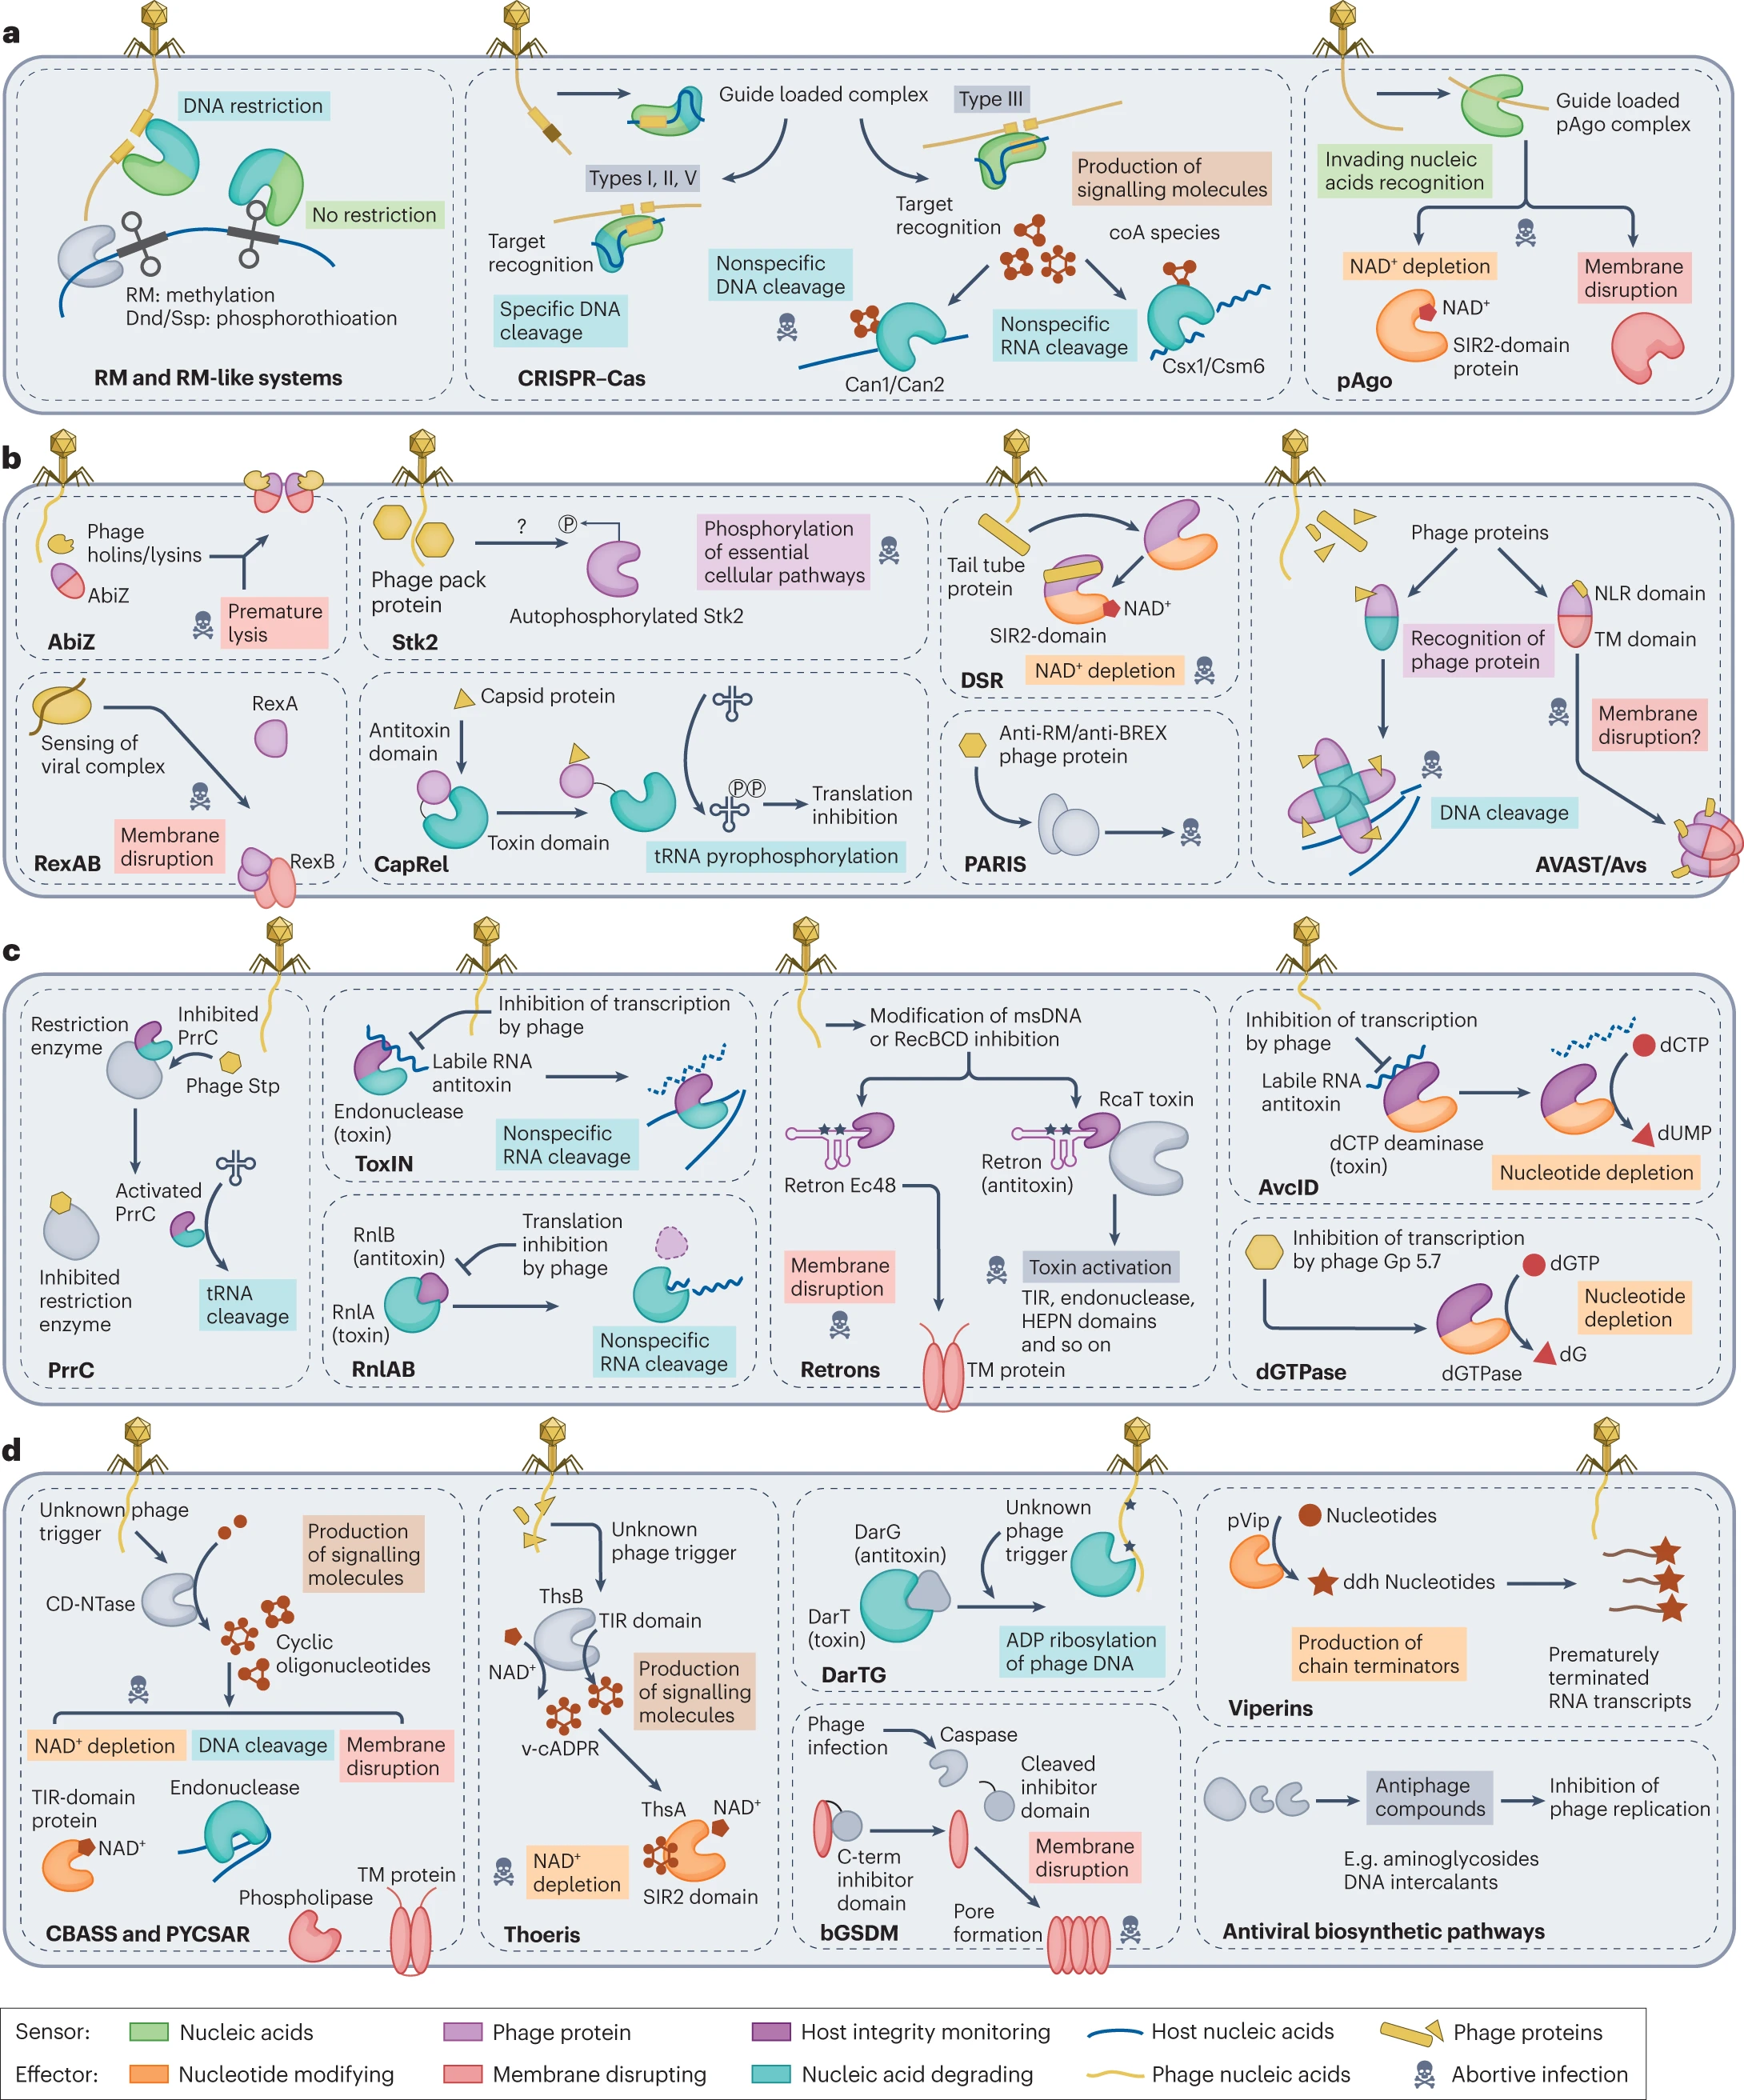
\includegraphics[width=\textwidth]{images/defensesys.png}
    \caption[Diversité des systèmes de défenses aux phages]{\textbf{Diversité des systèmes de défenses aux phages.} \textbf{a}) Systèmes de détection d'ADN étranger. \textbf{b}) Systèmes sensibles aux protéines phagiques. \textbf{c}) Systèmes de surveillance de l'intégrité de l'hôte. \textbf{d}) Autres mécanismes.  Extrait de \cite{georjon_highly_2023}}
    \label{fig:defsys}
\end{figure}

\newpage

Dans le même temps, avec l'émergence d'outils de détection (cf. \autoref{sec:defmet}), on s'intéresse à la distribution de ces systèmes dans les espèces procaryotes. Bernheim et Sorek \cite{bernheim_pan-immune_2020} ont montré qu'au sein d'une espèce toutes les souches ne présentent pas les mêmes systèmes et que les organismes s'échangent des systèmes par transfert horizontal. Cette propriété permet aux organismes de rapidement s'adapter aux phages présents dans l'environnement. Le système immunitaire doit donc être considéré comme l'ensemble des systèmes présents dans les organismes de l'environnement. En 2022, Tesson \textit{et al.} a montré que la composition en systèmes de défense varie entre les espèces, mais aussi selon la taille du génome, le risque d'infection et le mode de vie \cite{tesson_systematic_2022}. La composition en systèmes de défense est aussi étroitement liée aux phages qui peuvent infecter la bactérie, et réciproquement \cite{srikant_evolution_2022}. Pour terminer, Beavogui \textit{et al.} se sont intéressés au système immunitaire dans les données de génomique environnementale et ont montré une distribution différente des systèmes de défense en fonction de l'habitat et de la géographie \cite{beavogui_defensome_2024}.

Toutes ces études ont été permises par l'arrivée de méthodes et d'outils de détection automatique des systèmes de défense dans les génomes.

\subsubsection{Méthodes et outils de détection}
\label{sec:defmet}

Les premiers outils de détection dans les génomes, étaient spécialisés dans l'identification des systèmes CRISPR. Leur approche reposait sur la recherche de séquences répétées intercalées de séquences uniques, grâce à des méthodes d’alignement. PILER-CR \cite{edgar_piler-cr_2007} identifie d'abord toutes les séquences répétées palindromiques, sélectionne celles correspondant aux CRISPR (24 à 48 pb, séparées par des séquences uniques), puis affine leur détection grâce à une approche basée sur l’analyse de graphes et le partitionnement. L'outil CRT \cite{bland_crispr_2007}, utilise des k-mers pour rechercher des séquences répétées d'une taille donnée, éloignées d'une distance définie et dont la séquence est unique. Ces 2 méthodes sont rapides et ont l'intérêt de détecter toutes les séquences répétées candidates pour être des CRISPR. L'outil CRISPRFinder \cite{grissa_crisprfinder_2007}, va suivre un schéma similaire aux outils précédents, mais va introduire une notion de score, qui prend en compte le nombre de répétitions, leur taille, la régularité et la taille des espacements. De plus, une fois les séquences candidates filtrées, pour améliorer sa précision, CRISPRFinder peut comparer les candidats à sa base de données de CRISPRs validées.

Avec l'accumulation des connaissances autours des CRISPRs et des séquences environnantes qui les composent, les outils vont intégrer de nouveaux critères de détection. Des outils comme CRISPRstrand\cite{alkhnbashi_crisprstrand_2014}, CRISPRDirection\cite{biswas_accurate_2014} utilisent les séquences d'ARNcr\footnote{Les ARNcr, sont un type d'ARN contenant le transcrit d'une partie du CRISPR et le spacer. Ils sont utilisés dans la reconnaissance spécifique de l'ADN étranger.}, d'autres utilisent les séquences leader\footnote{Une séquence séparant les CRISPR des gènes codant pour les Cas.} comme CRISPRleader \cite{alkhnbashi_characterizing_2016}. La première version, MacSyFinder \cite{abby_macsyfinder_2014} intégrait une base de données HMM et de modèles CasFinder, pour identifier les protéines Cas et autres séquences connues proches pour identifier les systèmes CRISPR-Cas. En 2018, Une version hybride entre CRISPRFinder et CasFinder est proposé CRISPRCasFinder \cite{couvin_crisprcasfinder_2018}. Cet outil permet de prendre en compte la structure des CRISPR et des \textit{spacers}, ainsi que les gènes environnants, pour détecter finement les systèmes CRISPR-Cas.


En 2021, la découverte de nombreux nouveaux systèmes de défense a conduit au développement d’outils, comme PADLOC \cite{payne_identification_2021}, pour leur identification dans les génomes. PADLOC s’appuie sur une base de données HMM et de modèles décrivant les systèmes inspirés de la grammaire des modèles de MacSyFinder \cite{abby_macsyfinder_2014}. Peu après, DefenseFinder \cite{tesson_systematic_2022} a été publié, adoptant une approche méthodologique similaire reposant sur MacSyFinder pour la détection.
Bien que ces outils partagent un même principe de fonctionnement, ils diffèrent principalement dans la construction des profils HMM et dans les règles de détection des systèmes. PADLOC génère des HMMs entièrement \textit{de novo}, \textit{ie} qu'il construit sa propre base de données de profils, tandis que DefenseFinder s’appuie en partie sur des bases de données de protéines existantes, comme Pfam\cite{mistry_pfam_2021}. Par ailleurs, PADLOC privilégie une approche fondée sur des modèles plus généralistes, intégrant des règles plus flexibles afin de faciliter l’identification de systèmes proches de ceux connus. À l’inverse, DefenseFinder adopte des modèles plus stricts, intégrant un plus grand nombre de paramètres pour affiner la classification des systèmes identifiés.
Ainsi, le choix entre ces deux outils doit être guidé par les objectifs spécifiques de l’étude. PADLOC constitue une solution privilégiée pour les analyses exploratoires visant à détecter de nouveaux systèmes proches, tandis que DefenseFinder se révèle plus adapté aux études nécessitant une identification précise et rigoureuse des systèmes déjà caractérisés.

\section{Génomique à l'ère du Big Data}
\label{sec:db}
Avec l'évolution des méthodes de séquençage et la diminution des coûts, de plus en plus de projets de recherche s'appuient sur le séquençage des génomes pour faire des analyses de génomique comparée. Les chercheurs peuvent ensuite rendre ces séquences publiques et les déposer dans des banques de données (BD) de génomes, comme GenBank \cite{burks_genbank_1985}. GenBank est la BD de séquence du \textit{National Center for Biotechnology Information} (NCBI), toutes les séquences qui y sont soumises passent un contrôle d'intégrité et de qualité, avant d'être annotées automatiquement. Entre 2010 et 2025, le nombre de génomes stockés dans GenBank a connu une croissance exponentielle,  passant de quelques milliers à plus de 2,5 millions de génomes. (\autoref{fig:cumm_genbank}).

\begin{figure}[htbp]
    \centering
    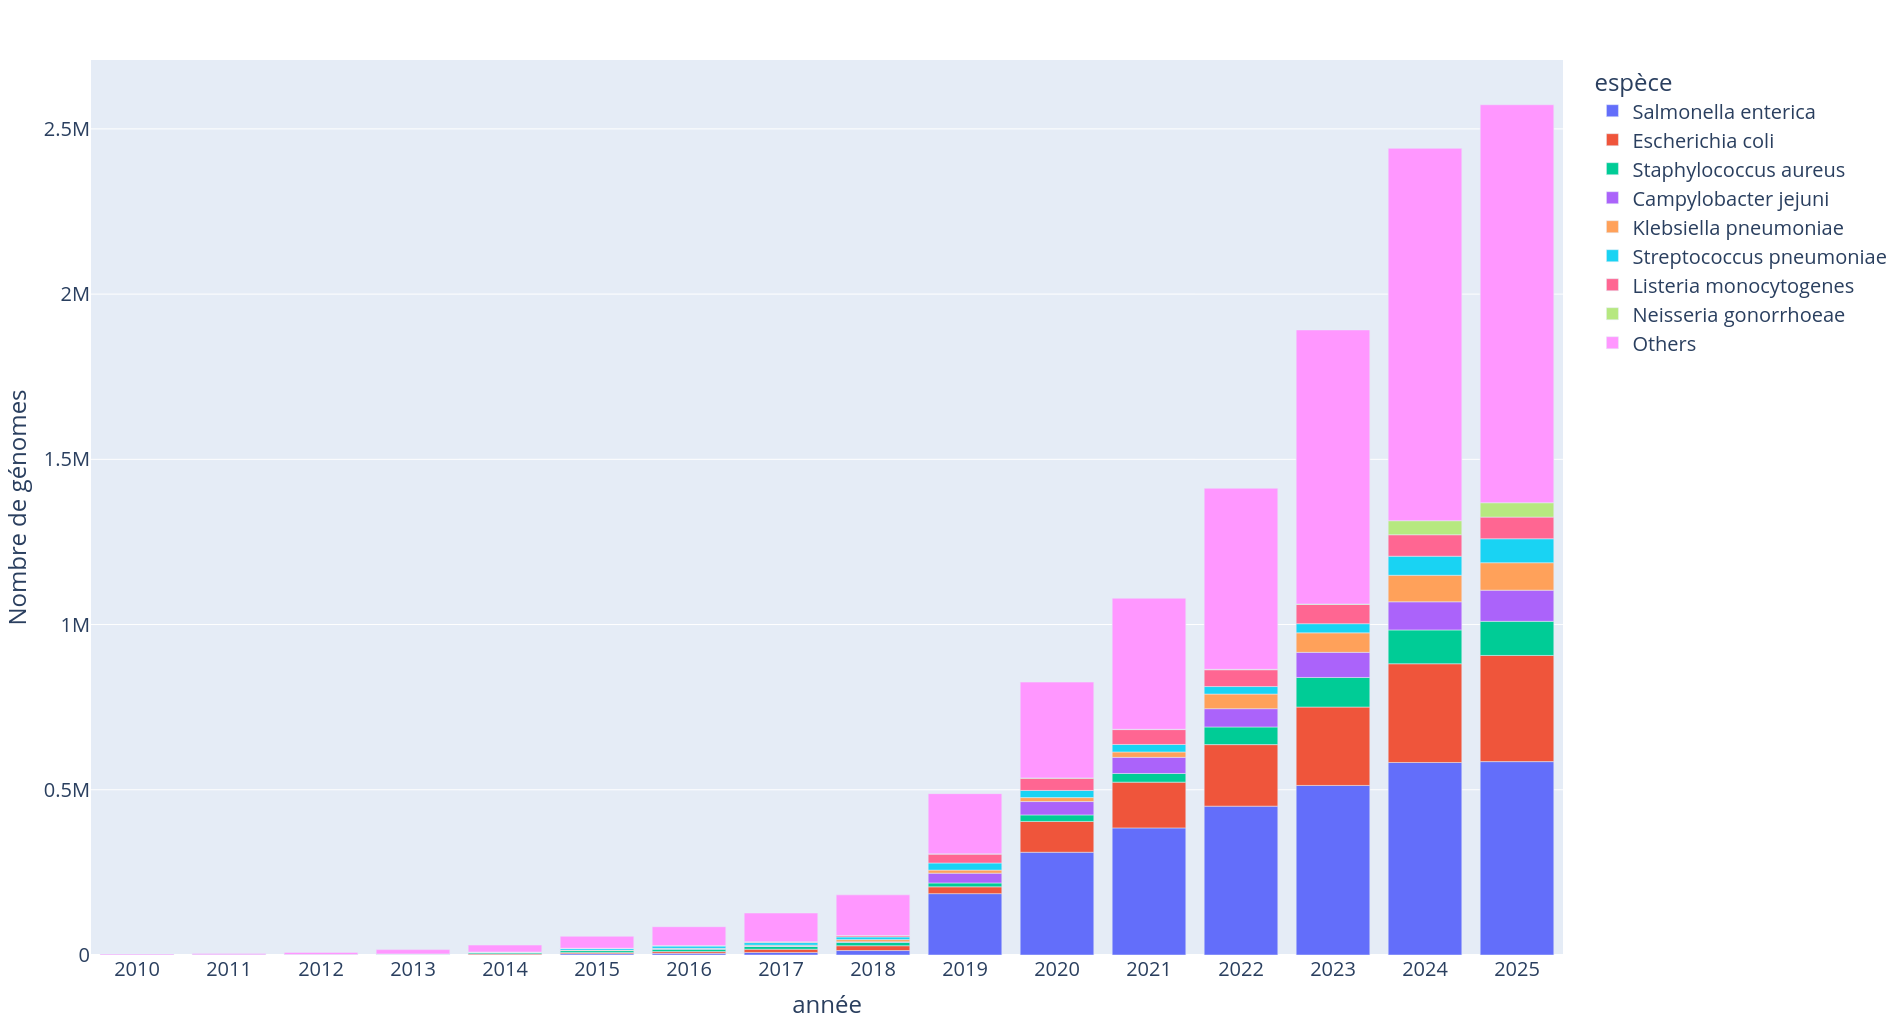
\includegraphics[width=\linewidth]{images/cummulativeGenomesGenBank.png}
    \caption[Nombre de génomes cumulés par an dans GenBank]{\textbf{Nombre de génomes cumulés par an dans GenBank.} Les génomes pris en compte sont uniquement ceux des procaryotes. Les espèces indiquées en légende sont les plus représentées dans GenBank. Construit avec l'outil drawbank \url{https://github.com/axbazin/drawbank}}
    \label{fig:cumm_genbank}
\end{figure}

À partir des génomes annotés, il est possible d'obtenir la traduction des gènes en séquences protéiques, prédire leurs fonctions, leurs structures\dots Toutes ces informations vont également être contenues dans des BD spécifiques pour aider aux analyses. Les BD peuvent aussi être thématiques, en contenant uniquement les génomes d'une espèce ou d'une région géographique, par exemple.

Avec l’essor du Big Data, les méthodes de génomique comparée vont être améliorées et adaptées afin d'analyser efficacement ce nouvel immense volume de données.
%La génomique doit alors s'adapter et profiter de ce vaste ensemble de données qu'est le \textit{Big Data}.

\subsection{Base de données génomiques}

L’existence et l’accessibilité des bases de données biologiques sont fondamentales pour l’annotation, la classification et l’analyse des séquences génomiques et protéiques. Parmi ces ressources, plusieurs se distinguent par leur spécialisation.

Parmi les bases de données de référence de génomes, RefSeq \cite{pruitt_ncbi_2007}, développée et maintenue par le NCBI, se distingue par la qualité et la fiabilité de ses annotations. Contrairement à GenBank, alimentée par des soumissions d’utilisateurs, RefSeq compile des séquences rigoureusement validées, incluant des ARN et des protéines issus d’une grande diversité d’organismes. Son processus de standardisation strict en fait une ressource incontournable pour la génomique comparative et une base essentielle pour des outils phares du NCBI, comme BLAST. En complément des séquences individuelles, RefSeq propose des ensembles complets de génomes annotés, notamment pour des organismes modèles et des pathogènes.

Dans le domaine des protéines, \textbf{UniProt} \cite{the_uniprot_consortium_uniprot_2025} est une ressource incontournable pour l’annotation et l’analyse des séquences protéiques. Elle est développée et maintenue par un consortium composé de l'\textit{European Bioinformatics Institute }(EMBL-EBI), le \textit{Swiss Institute of Bioinformatics} (SIB) et la \textit{Protein Information Resource} (PIR). Elle se divise en 3sections : (\textit{i}) \textbf{UniProtKB} (\textit{KnowledgeBase}), qui comprend des annotations détaillées sur les protéines et est divisé en \textbf{Swiss-Prot} (annotations manuelles et validées) et \textbf{TrEMBL} (annotations automatiques) \cite{apweiler_uniprot_2004,bairoch_swiss-prot_2004} ; (\textit{ii}) \textbf{UniRef} (\textit{UniProt Reference Clusters}), qui regroupe des séquences non redondantes à différents seuils de similarité \cite{suzek_uniref_2007}; (\textit{iii}) \textbf{UniParc} (\textit{UniProt Archive}), une archive complète de toutes les séquences protéiques connues, indépendamment de leur source. Cette base de données est essentielle pour la modélisation structurale des protéines, la découverte de cibles thérapeutiques et la génomique fonctionnelle.

\textbf{GTDB} (Genome Taxonomy Database) \cite{parks_standardized_2018} propose une taxonomie révisée des génomes procaryotes, fondée sur des analyses phylogénomiques. Contrairement aux approches classiques reposant sur des critères phénotypiques, GTDB utilise une approche purement génomique basée sur l'analyse comparée de 120 gènes marqueurs afin d’harmoniser la classification. Comme l’illustre la \autoref{fig:GTDB_tax}, cette approche permet d’obtenir une taxonomie plus homogène que celle du NCBI. De plus, GTDB intègre les génomes environnementaux et non cultivables issus de métagénomes, facilitant ainsi l’identification de nouvelles espèces et l’exploration de la diversité microbienne selon des critères plus objectifs.

\begin{figure}
    \centering
    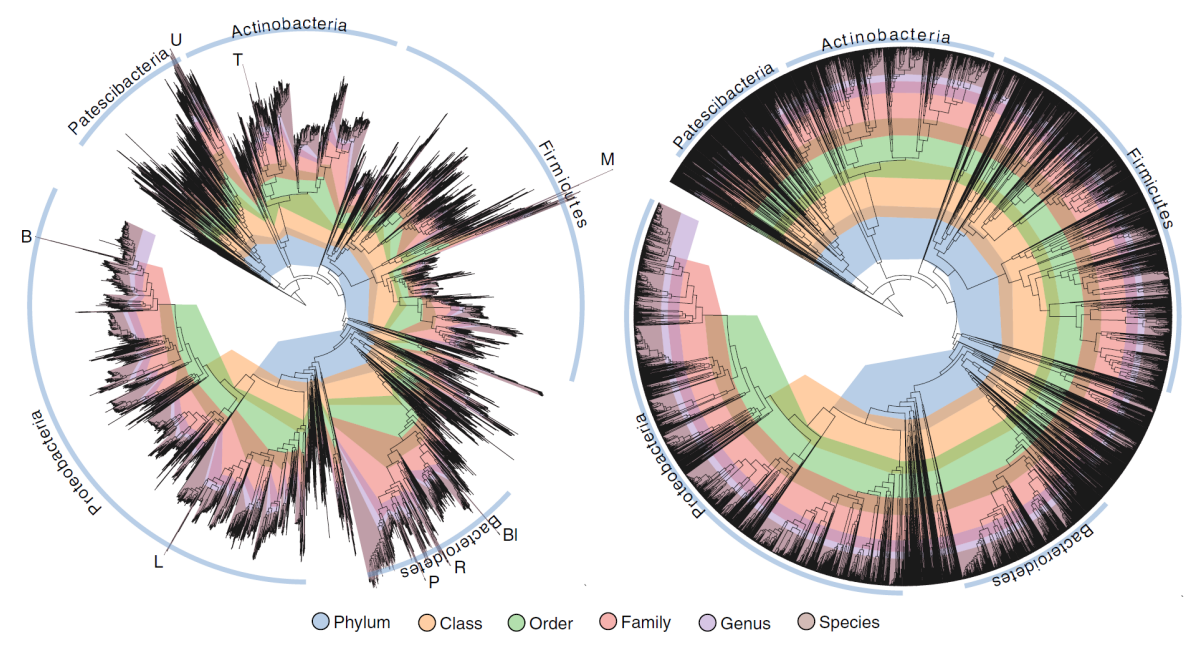
\includegraphics[width=.75\linewidth]{images/GTDB_taxonomie.png}
    \caption[Comparaison de l'homogénéité des rangs taxonomiques entre le NCBI et GTDB]{\textbf{Comparaison de l'homogénéité des rangs taxonomiques entre le NCBI et GTDB.} Les 2 figures représentent le même arbre avec à gauche la taxonomie proposée par le NCBI et à droite celle proposée par GTDB. Copié de \cite{gautreau_conceptualisation_2020} et adapté de \cite{parks_standardized_2018}}
    \label{fig:GTDB_tax}
\end{figure}

L’analyse des communautés microbiennes complexes repose sur des bases de données spécialisées comme \textbf{MGnify}\footnote{anciennement nommé EBI Metagenomics \cite{hunter_ebi_2014}} \cite{richardson_mgnify_2023}, une plateforme développée par l’EMBL-EBI dédiée à l’étude des données métagénomiques. Contrairement aux bases centrées sur des séquences génétiques isolées, MGnify s’intéresse aux microbiomes présents dans divers environnements tels que le sol, les océans, les eaux douces, le microbiote humain ou encore les milieux extrêmes. En plus de stocker des données, elle propose des outils bioinformatiques avancés pour l’assemblage, l’annotation et l’analyse fonctionnelle des communautés microbiennes. MGnify permet ainsi d’identifier les espèces présentes dans un échantillon via des approches de taxonomie basées sur l’ARNr 16S/18S, de prédire les fonctions métaboliques des microbiomes et d’étudier leurs interactions avec l’environnement. Cette ressource est devenue incontournable en écologie microbienne et en biotechnologie.

Dans le domaine de la résistance aux antibiotiques, CARD (\textit{Comprehensive Antibiotic Resistance Database}) \cite{mcarthur_comprehensive_2013} est une base de données spécialisée qui regroupe des informations sur les gènes de résistance, les mutations associées et les mécanismes moléculaires impliqués. Elle est notamment utilisée pour identifier les gènes de résistance dans des échantillons génomiques en utilisant l'outil RGI \cite{alcock_card_2023}, et métagénomiques grâce à l’outil CARPDM \cite{hackenberger_carpdm_2024}. CARD adopte une nomenclature standardisée basée sur l’ontologie ARO (\textit{Antibiotic Resistance Ontology}) pour classifier les résistances selon leur mode d’action et leur mode de transmission, facilitant ainsi l’étude et la surveillance des résistances aux antibiotiques.

Enfin, pour les chercheurs spécialisés dans l'étude des bactéries du genre Pseudomonas, la \textbf{Pseudomonas Genome Database} (PGD) constitue une ressource précieuse \cite{winsor_enhanced_2016}. Cette base de données centralise des informations sur le séquençage et l’annotation des génomes des différentes espèces de Pseudomonas, un groupe bactérien d’importance en médecine, en agriculture et en biotechnologie. PGD fournit des annotations génomiques détaillées, des informations fonctionnelles et des descriptions précises des voies métaboliques. De plus, les données y sont validées par des experts du domaine. La plateforme permet également des analyses comparatives entre souches, offrant ainsi un outil puissant pour l’étude de la diversité génétique et fonctionnelle de ces bactéries.

Chacune de ces bases de données joue un rôle clé dans l’analyse des génomes et des protéines, en apportant des solutions adaptées aux besoins des microbiologistes. Leur complémentarité permet une exploration approfondie des données biologiques et contribue aux avancées scientifiques dans de nombreux domaines.

\subsection{Bases de données orientées graphe et données biologiques}

Les premières bases de données biologiques ont été construites sur un modèle relationnel, fondé sur l’organisation des données en tables où chaque ligne représente un élément et chaque colonne un attribut de cet élément. Pour établir des relations entre ces entités, chaque élément se voit attribuer un identifiant unique, qui est ensuite utilisé dans des tables de correspondance reliant différents éléments entre eux. Ce modèle s’avère particulièrement pertinent lorsque les données sont relativement stables et que les relations entre éléments sont peu nombreuses et secondaires par rapport aux attributs eux-mêmes. Il permet ainsi de stocker efficacement un génome et ses métadonnées associées, telles que l’organisme d’origine, le laboratoire de séquençage, la date d’obtention ou encore les publications qui y sont liées.

Toutefois, avec l’accroissement massif des données biologiques, ces BD relationnelles, appelées aussi SQL\footnote{SQL réfère au langage de requête de ces bases, mais par abus de langage, on parle de base SQL}, atteignent leurs limites. Lorsque les données deviennent extrêmement connectées, interroger ces BD nécessite des requêtes complexes et des ressources computationnelles importantes, ce qui peut ralentir l’accès et l’analyse des informations \cite{hsu_correlation_2014}. Pour pallier ces contraintes, de nouveaux modèles émergents, privilégiant une approche non seulement relationnelle (NoSQL). Il existe plusieurs types de BD NoSQL, ici, nous nous focaliserons sur un type particulier : les bases de données orientées graphe (BDG).

Contrairement aux bases relationnelles, les BDG modélisent les données sous forme de graphes, où les n\oe uds représentent les éléments et les arêtes définissent leurs relations. Ce modèle offre une représentation plus intuitive des connexions complexes, ce qui est particulièrement utile pour l’analyse des réseaux biologiques, comme les interactions entre protéines, les relations entre gènes ou encore les mécanismes de résistance aux antibiotiques. De plus, bien que ces bases reposent sur une structure différente, il reste possible de traduire un graphe en une base relationnelle, comme illustré sur la \autoref{fig:DBRel_vs_Graph}.

\begin{figure}[htbp]
    \centering
    \subfloat[Base de données relationnelle]{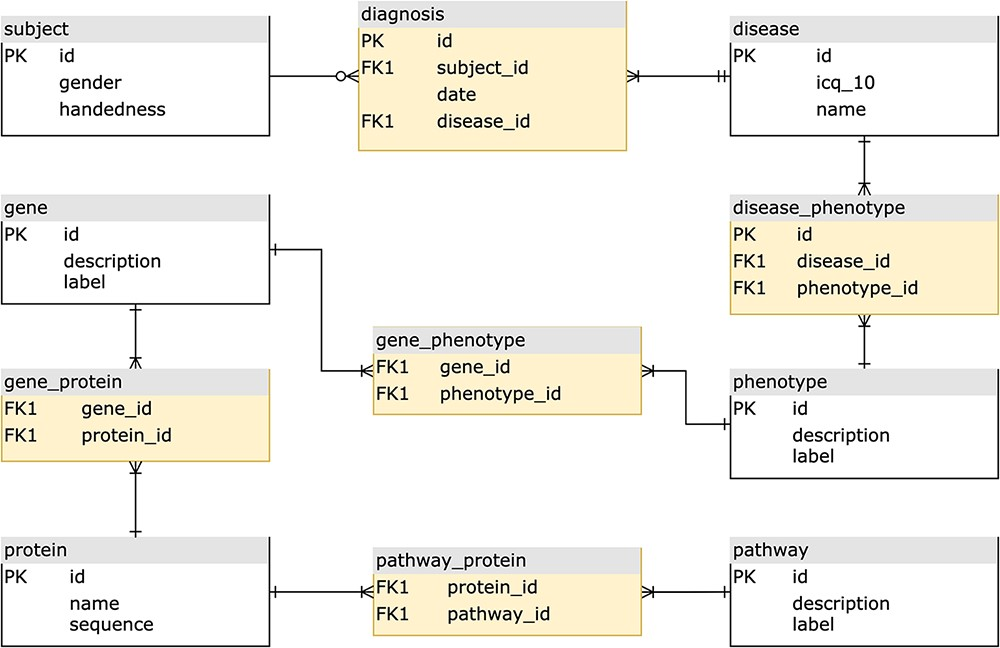
\includegraphics[width=0.5\linewidth]{images/DBRel.jpeg}}
    \hfill
    \subfloat[Base de données graphe]{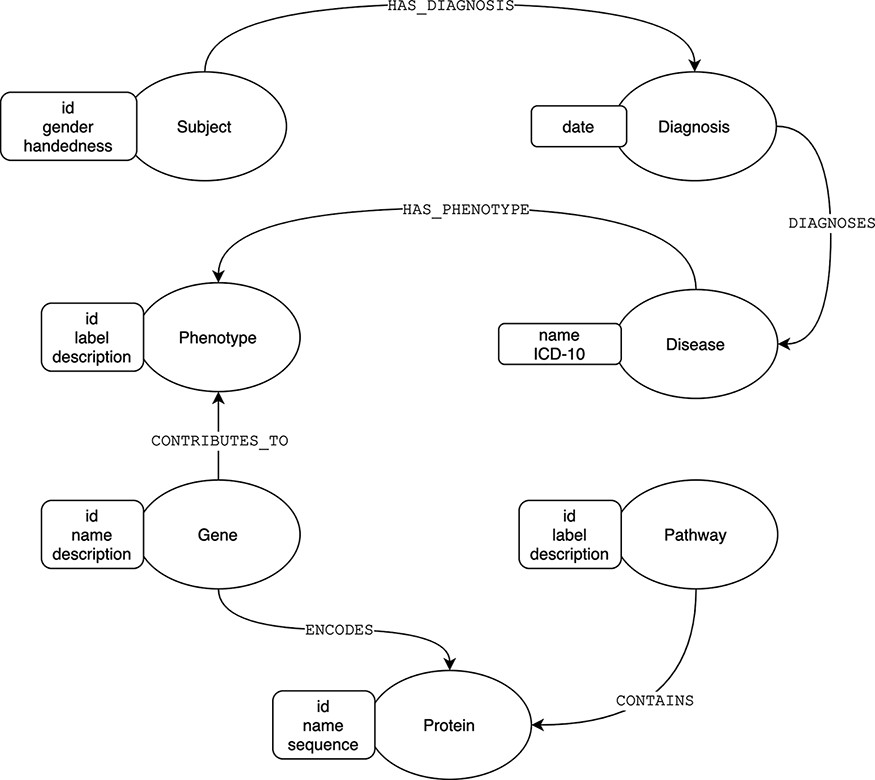
\includegraphics[width=0.4\linewidth]{images/DBGraph.jpeg}}
    \caption[Comparaison des modèles entre une base de données relationnelle et une base de données orientées graphe]{\textbf{Comparaison des modèles entre une base de données relationnelle et une base de données orientées graphe.} (a) Les tables contenant les informations sont représentées en blanc et les tables de jointure en jaune. (b) Les n\oe uds représentent les informations et les arêtes les relations (jointure). Extrait de \cite{timon-reina_overview_2021}}
    \label{fig:DBRel_vs_Graph}
\end{figure}

Parmi les bases de données et outils qui exploitent ces nouveaux modèles, GDM (Genomic Data Model) et GMQL (Genomic Metadata Query Language) illustrent bien l’évolution vers des architectures plus flexibles adaptées aux vastes ensembles de données génomiques \cite{masseroli_genometric_2015,masseroli_modeling_2016}. GDM est un modèle conçu pour gérer efficacement des données hétérogènes issues de la génomique, en intégrant à la fois des informations sur les séquences et leurs annotations. Dans cette perspective, GMQL se présente comme un langage de requête avancé permettant d’interroger ces bases de manière optimisée, facilitant l’exploration et l’intégration de données. Grâce à son interaction avec un modèle orienté graphe, GMQL améliore la capacité à interroger et à analyser de grands ensembles de données interconnectées, rendant possible l’identification rapide de corrélations complexes entre différentes sources d’information génomique.

\newpage

Dans le domaine du Web sémantique, BioRDF \cite{cheung_journey_2009} permet de modéliser et d'interconnecter des ressources issues des DB, biomédicales en particulier. Reposant sur le \textit{Ressource Description Framework} (RDF), cette approche permet de relier des concepts biologiques de manière standardisée, permettant ainsi une interopérabilité accrue entre les systèmes et l’extraction de nouvelles connaissances à partir de réseaux complexes. RDF est un modèle de données qui représente l'information sous forme de graphes. Chaque déclaration RDF est un triplet composé d'un sujet, d'un prédicat et d'un objet, ce qui forme naturellement une structure de graphe. BioRDF est utilisé dans diverses applications biologiques, y compris la création de \textit{workflows} bioinformatiques, l'annotation de séquences protéiques, et la modélisation de voies biologiques. Des outils comme Taverna \cite{oinn_taverna_2004} sont utilisés pour composer et exécuter ces workflows.

Un autre exemple de base de données orientée graphe est KEGG (\textit{Kyoto Encyclopedia of Genes and Genomes}), une ressource essentielle pour l’analyse des voies métaboliques, des interactions moléculaires et des relations entre gènes et maladies \cite{kanehisa_kegg_2025}. Contrairement aux bases relationnelles classiques, KEGG structure ses données sous forme de graphes de réseaux métaboliques, où les n\oe uds représentent des gènes, des protéines ou des petites molécules, interconnectés à travers des réactions biochimiques représentées par les arêtes. Cette organisation permet d’étudier le fonctionnement des systèmes biologiques à grande échelle et d’identifier des cibles potentielles pour le développement de nouvelles thérapies.

Ces bases de données sont également utilisées par des outils pour réaliser des analyses et des prédictions. C'est le cas de Spfy \cite{le_spfy_2018}, qui permet de prédire des phénotypes bactériens sur de nouveaux échantillons à partir d'une base de données MongoDB\footnote{MongoDB, une base orientée documents, adapté aux ensembles de données évolutifs et hétérogènes.} \cite{guo_mongodbs_2017}. Spfy est capable de prédire des caractéristiques phénotypiques importantes telles que le sérotype, le sous-type de la toxine Shiga (toxine sécrétée par les bactéries \textit{E. coli}), ainsi que la présence de facteurs de virulence et de déterminants de résistance aux antimicrobiens. Actuellement, la base de données contient plus de 10 000 génomes de \textit{Escherichia coli}.

Enfin, l’utilisation des bases de données orientées graphe s’est intensifiée avec des systèmes de gestion de base de données orientée graphe open-source comme Neo4J, qui a été largement exploité dans des projets tels que CovidGraph \cite{gutebier_covidgraph_2022}. Ce dernier est un réseau de connaissances conçu pour analyser la littérature scientifique, les bases de données biomédicales et les publications liées au SARS-CoV-2. En structurant ces informations sous forme de n\oe uds et d’arêtes, Neo4J permet d’explorer efficacement les relations complexes entre les études, les auteurs, les interactions moléculaires et les traitements potentiels contre la maladie.

Ces nouvelles approches et ces outils illustrent la transition vers des modèles de bases de données plus dynamiques et adaptés aux défis de la biologie moderne. Que ce soit par l’utilisation de langages de requête spécialisés, de technologies sémantiques, de modèles en graphe ou encore de bases NoSQL, ces solutions permettent une gestion plus efficace des données biomédicales et ouvrent la voie à des analyses plus approfondies dans le domaine des sciences de la vie.


\subsection{L'intelligence artificielle au service de la génomique comparée}

\subsubsection{Définitions et concepts}

Avec l’accumulation massive de données, la génomique est désormais confrontée aux défis du \textit{Big Data}, tant en termes de volume que de complexité. Les bioinformaticiens se tournent donc vers des méthodes développées dans la science des données (\textit{data science}) et particulièrement vers l'intelligence artificielle (IA). L’intelligence artificielle regroupe un ensemble de techniques permettant aux machines de reproduire certaines facultés cognitives humaines, telles que l’apprentissage, le raisonnement et la résolution de problèmes. Elle s’appuie sur divers domaines de recherche définissant le traitement des données, la prise de décision et l’adaptation des algorithmes aux informations reçues. Ici, nous nous intéresserons à un champ de recherche particulièrement utilisé en bioinformatique, celui de l'apprentissage automatique (\textit{machine learning en anglais}, ML). 

Les méthodes de ML correspondent à des méthodes qui s'améliorent par l'apprentissage ou l'entraînement. Pour fonctionner, elles ont besoin de grands jeux de données, bien définis. Elles sont donc bien adaptées à la génomique du Big Data. Dans une application de ML (\autoref{fig:ML_base}), après avoir bien défini les données d'entrée et la prédiction attendue, une phase d'apprentissage permet de construire le modèle le plus adapté. La première étape de l'apprentissage consiste à entraîner le modèle sur un jeu de données (d’entraînement) pour sélectionner les caractéristiques les plus pertinentes et estimer les meilleurs paramètres du modèle. Une deuxième étape d'évaluation (ou de test) mesure les performances du modèle, \textit{i.e.}, la divergence avec le résultat attendu\footnote{Cette divergence est mesurée par la fonction de perte ou de coût}. En fonction de l'évaluation, un nouvel apprentissage peut être relancé pour améliorer le modèle. Même si le modèle ne sera jamais idéal, le choix des jeux d’entraînement et de test permet de s'approcher au mieux de la prédiction souhaitée. 

\begin{figure}[htbp]
    \centering
    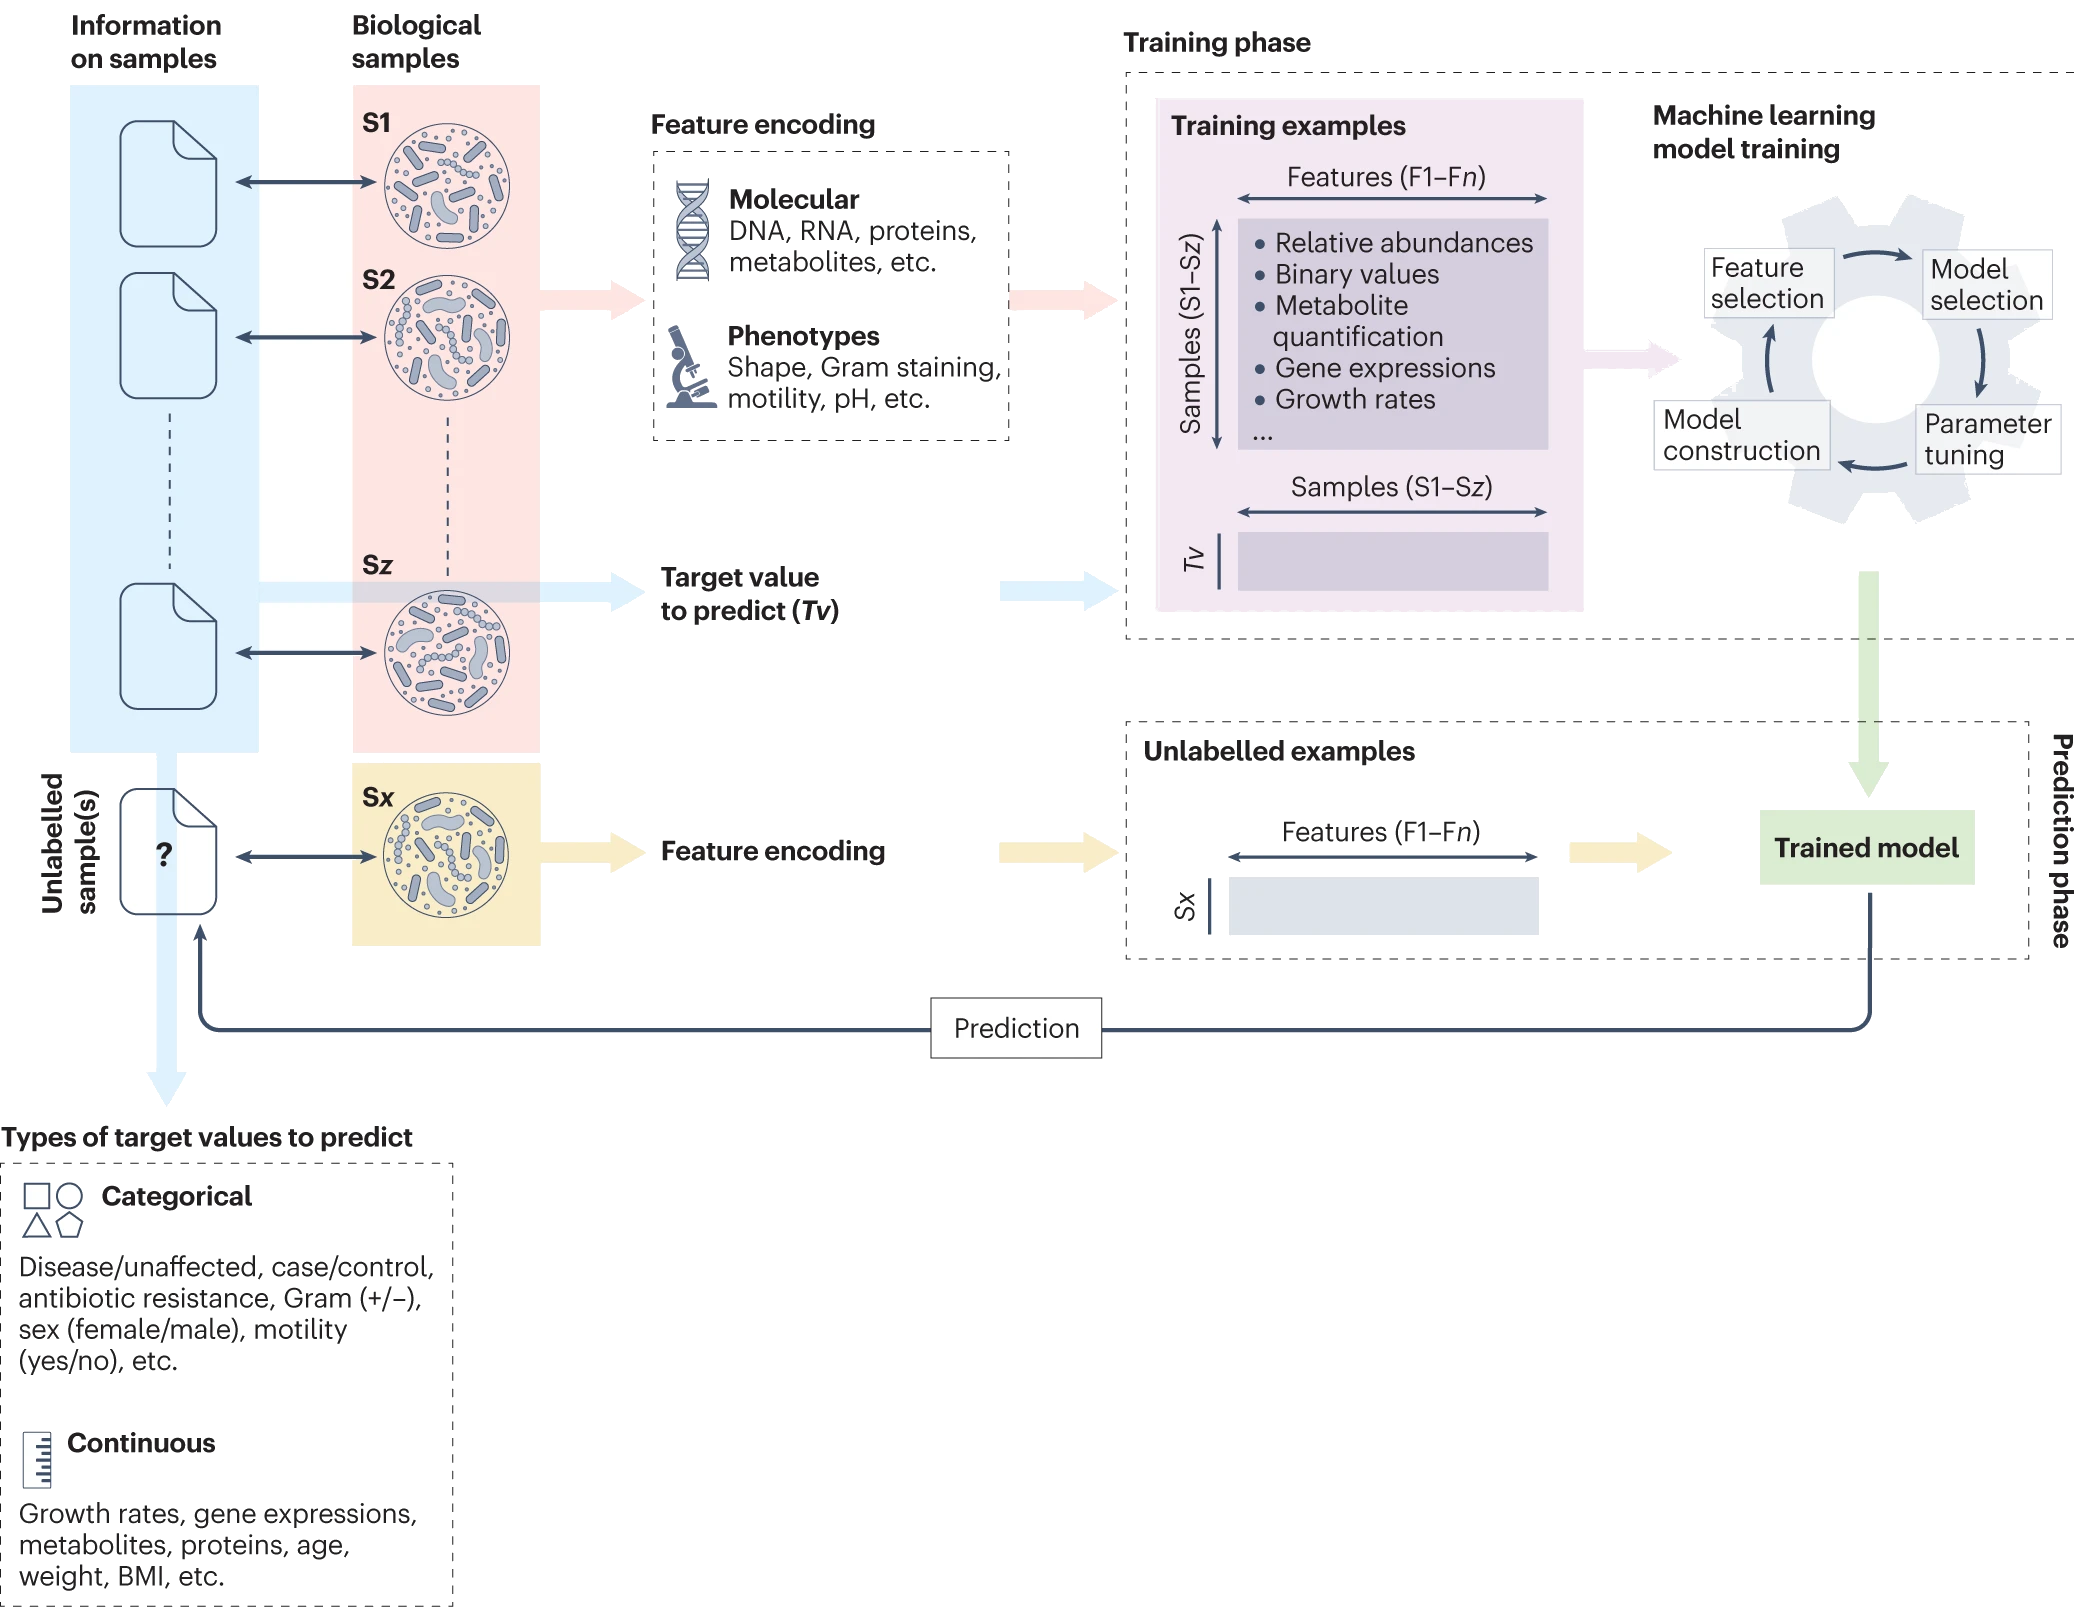
\includegraphics[width=\linewidth]{images/ML.png}
    \caption[Schéma général d'une application de machine learning]{\textbf{Schéma général d'une application de machine learning pour l'assignation de caractéristiques moléculaires et phénotypiques.} Le schéma correspond à l'application d'un modèle supervisé où les données d'entrée sont étiquetées et dont la prédiction attendue est, elle aussi, une étiquette. Extrait de \cite{asnicar_machine_2024}}
    \label{fig:ML_base}
\end{figure}

\newpage

Les méthodes de machine learning peuvent être divisées en 2 grandes catégories : (\textit{i}) l'apprentissage \textbf{supervisé}; (\textit{ii}) l'apprentissage \textbf{non supervisée}. 

Les modèles supervisés permettent d'assigner des \textbf{étiquettes} aux données. Dans ce cas, les données du jeu d’entraînement et de test sont étiquetées par le résultat attendu (à priori). La \autoref{fig:ML_base}, présente un ensemble d'échantillons dont on possède les informations d'intérêt. Le modèle entraîné est appliqué sur un nouvel échantillon et permet donc de prédire les informations jusqu'alors inconnues. Par exemple, en entraînant un classificateur supervisé (tel qu’un modèle de régression) sur des assignations génome-espèce connues, et en utilisant la présence ou l’absence de gènes marqueurs comme caractéristiques, il devient possible d’attribuer une taxonomie à un nouveau génome.

Les modèles non supervisés permettent de rechercher des structures dans des données sans nécessité d'étiquettes. Dans ce cas, après la phase d’entraînement, il y a une autoévaluation du modèle basée sur un renforcement positif. Par exemple, si l'on s'intéresse aux gènes impliqués dans la croissance bactérienne, les modèles peuvent partitionner les groupes de gènes présentant des profils d'expression génique similaires reflétant la croissance cellulaire. Les modèles non supervisés ont l'intérêt de pouvoir résoudre des problèmes plus complexes, sans avoir besoin de données annotées ; par contre, ils sont beaucoup plus imprévisibles que les modèles supervisés.

\begin{figure}[htbp]
    \centering
    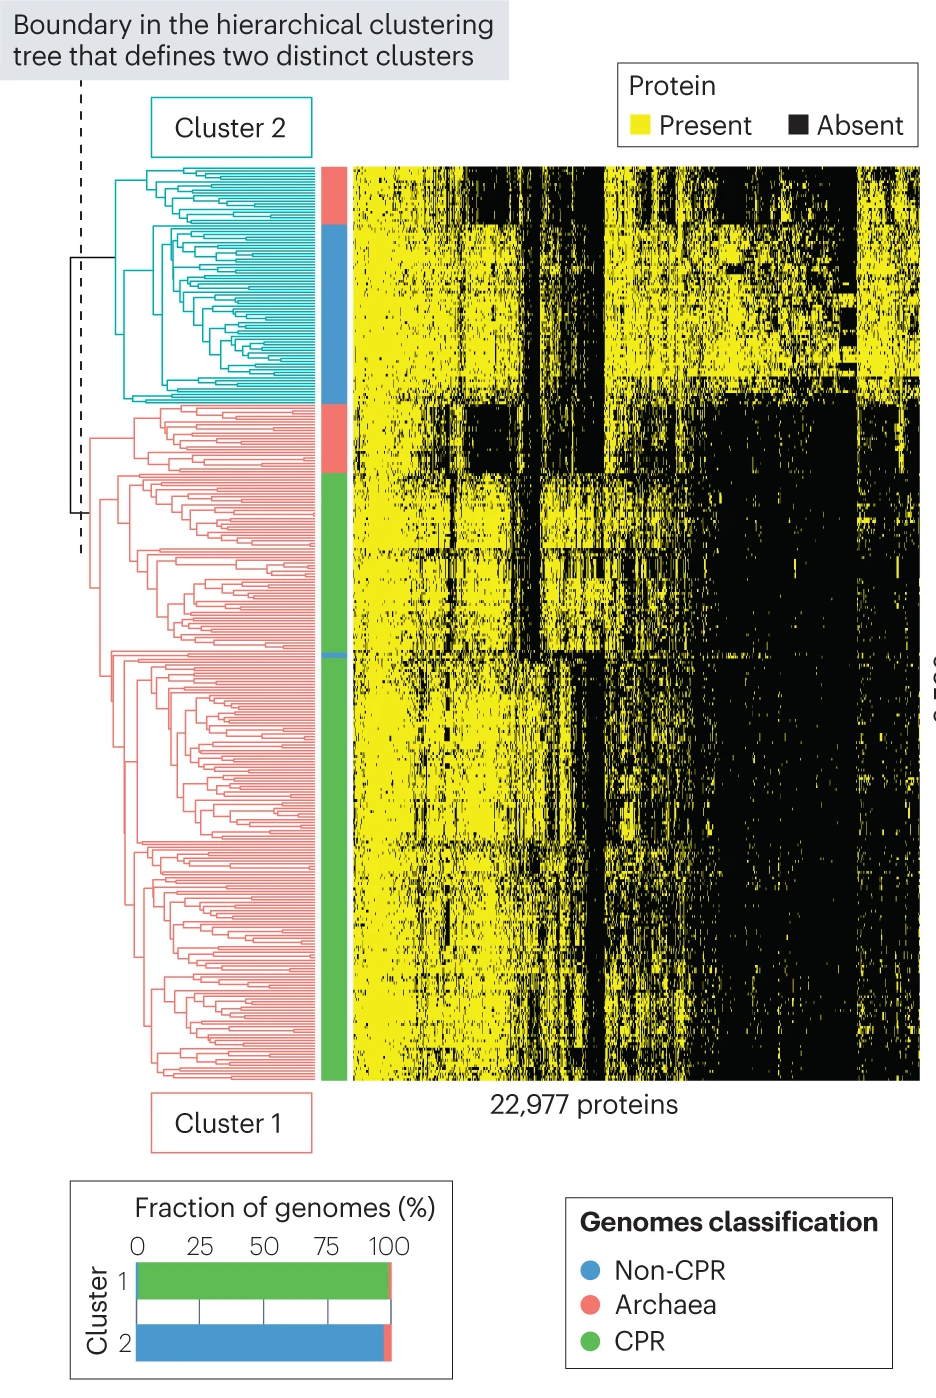
\includegraphics[width=0.5\linewidth]{images/hierachical_clustering.png}
    \caption[Exemple d'application de méthode non supervisé]{\textbf{Exemple d'application de méthode non supervisée.} Le \textit{HeatMap} représente pour chaque souche la présence/absence d'un ensemble de protéines. La méthode de clustering (ici une Analyse en composantes principales) permet d'identifier 2 groupes dans les souches, correspondant à 2 groupes taxonomiques. Extrait et adapté de \cite{asnicar_machine_2024}}
    \label{fig:enter-label}
\end{figure}

Dans les années 2010, un sous-domaine de l'apprentissage automatique gagne en popularité, l'apprentissage profond (\textit{deep learning} en anglais DL)\footnote{Les premières approches de DL datent des années 1940. Le terme regagne en popularité en 2006 suite à l'article de Geoffrey Hinton and Ruslan Salakhutdinov \cite{hinton_fast_2006}}. Les algorithmes de DL sont basés sur le concept de \textbf{réseaux neuronaux} (artificiels). Ces réseaux peuvent être représentés sous forme d'un graphe orienté, pondéré et étiqueté, comme sur la \autoref{fig:reseaux}. Ce réseau est organisé en couches successives, avec une couche d'entrée (à gauche) correspondant aux données brutes, des couches cachées (au centre) qui effectuent des transformations des données et extraient des caractéristiques, et enfin une couche de sortie (à droite) qui contient la prédiction. L'intérêt du DL réside dans sa capacité à extraire automatiquement les caractéristiques pertinentes lorsque les données passent dans les couches cachées. Plus le nombre de couches est élevé, plus le modèle peut apprendre, plus les questions que l'on pose peuvent être complexes et les réponses précises. Cependant, en augmentant la complexité, on augmente aussi la difficulté d'interprétation\footnote{On parle parfois de boite noire dans les modèles les plus complexes dans le sens où, dans les couches cachées, il est souvent difficile de savoir comment les données ont été transformées et classées.}. 

\begin{figure}
    \centering
    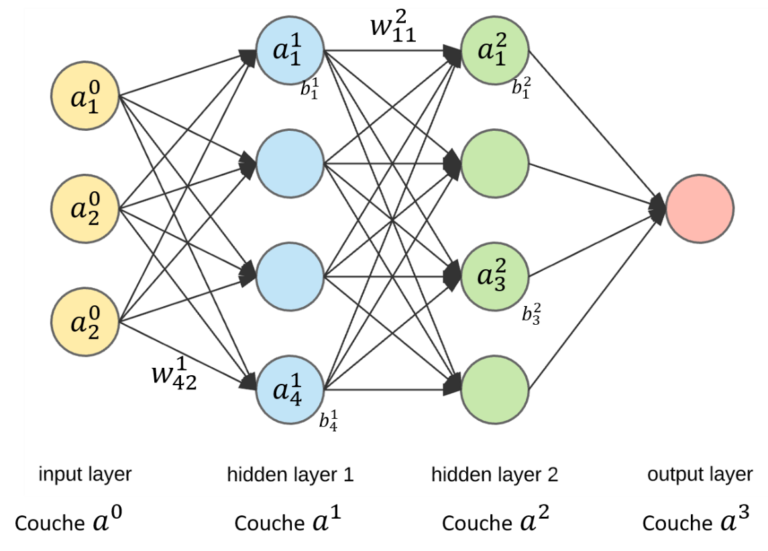
\includegraphics[width=0.5\linewidth]{images/reseaux_neurone.png}
    \caption[Représentation d'un réseau de neurone à 3 couches]{\textbf{Représentation d'un réseau de neurones à 3 couches.} Extrait de \url{https://www.aspexit.com/reseau-de-neurones-on-va-essayer-de-demystifier-un-peu-tout-ca-1/}}
    \label{fig:reseaux}
\end{figure}

Réaliser une étude de ML/DL peut être un problème épineux. Il faut d'abord avoir une bonne compréhension des données pour s'orienter vers des méthodes supervisées ou non, et choisir entre l'apprentissage traditionnel et profond (cf. \autoref{tab:ML_met} 
\& \autoref{tab:dl_met}). Il convient également de s'assurer de la qualité des données ; si le modèle apprend sur des données corrompues, les prédictions seront fausses. Ceci fait, on choisit un modèle et des paramètres, dont on évalue les performances. L'indicateur doit être choisi judicieusement pour refléter correctement l'efficacité du modèle. L'évaluation du modèle doit aussi être reproductible, \textit{i.e.} testée sur de nouveaux jeux de données via des approches comme la validation croisée entre ensembles distincts. Un autre point d'attention est celui du sur-apprentissage (\textit{overfitting} en anglais). Un modèle trop complexe risque de capturer non seulement les relations sous-jacentes, mais aussi le bruit des données, menant ainsi à des résultats biaisés. Tous ces points sont suffisamment importants pour que finalement "Le choix d'un algorithme d'apprentissage automatique particulier [est] moins important que son application et son utilisation correctes et différents algorithmes d'apprentissage automatique appliqués de la bonne manière devraient fournir des résultats cohérents." \cite{asnicar_machine_2024}.

\begin{table}[htbp]
    \centering
    % \footnotesize
    \small
    \begin{sideways}
    \begin{tabular}{|>{\raggedright\arraybackslash}p{0.1\textheight}|>{\raggedright\arraybackslash}p{0.1\textheight}|>{\raggedright\arraybackslash}p{0.15\textheight}|>{\raggedright\arraybackslash}p{0.275\textheight}|>{\raggedright\arraybackslash}p{0.275\textheight}|}
    \hline
    \textbf{Méthode} & \textbf{Type de données} & \textbf{Exemples d'applications} & \textbf{Avantages} & \textbf{Inconvénients} \\
    \hline
    Régression Ridge (et LASSO / élastique) & \multirow{5}{0.1\textheight}[-5em]{Étiquetées Nombre de caractéristiques fixe} & Prédiction de l'expression des gènes en réponse à des antibiotiques & Facile à interpréter \newline Facile à entraîner \newline Bon benchmark & Ne peut pas apprendre des relations complexes entre caractéristiques \newline Sur-apprend avec un grand nombre de caractéristiques \\
    \cline{1-1}\cline{3-5}
    Machine à vecteurs de support & & Classification des gènes en fonction de leur fonction & Peut effectuer à la fois la classification et la régression linéaire et non linéaire & Difficile à adapter à de grands ensembles de données \\    
    \cline{1-1}\cline{3-5}
    Forêt aléatoire &  & Identification des mutations génomiques associées à un phénotype & Apprend l'importance de chaque caractéristique pour la prédiction \newline Les arbres de décision individuels sont lisibles par l'humain \newline Moins sensible à l'échelle et à la normalisation des caractéristiques, donc plus facile à entraîner et à ajuster & Moins approprié pour la régression \newline De nombreux arbres de décision sont difficiles à interpréter \\     
    \cline{1-1}\cline{3-5}
    Boosting de gradient (ex. XGBoost) & & Profilage de l'expression des gènes & Apprend l'importance de chaque caractéristique \newline Arbres de décision lisibles par l'humain Moins sensible à l'échelle et à la normalisation & Peut avoir du mal à apprendre le signal sous-jacent en présence de bruit Moins adapté à la régression \\
    \hline
    Clustering & Non étiquetées \newline Nombre de caractéristiques fixe & Groupement des gènes bactériens en fonction de leurs profils d'expression dans différentes conditions environnementales & Bon clustering facilement identifiable pour les données de faible dimension \newline Métriques de validation de clustering disponibles & Difficile à appliquer à de grands ensembles de données \newline Les ensembles de données bruités peuvent produire des résultats contradictoires \\     
    \hline
    Réduction de dimensionnalité & Non étiquetée Grand nombre de caractéristiques fixe & Visualisation des relations entre différentes souches bactériennes basées sur leurs génomes & Fournit une représentation visuelle des données Évaluations de l'ajustement souvent disponibles & Difficile de préserver à la fois les différences locales et globales Difficile à appliquer à un grand nombre d'échantillons \\        
    \hline
    \end{tabular}
    \end{sideways}
    \caption[Méthodes de Machine learning]{\textbf{Méthodes de Machine learning.} Extrait et adapté de \cite{greener_guide_2022}}
    \label{tab:ML_met}
\end{table}

\begin{table}[htbp]
    \centering
    \small
   \begin{sideways}
   \begin{tabular}{|>{\raggedright\arraybackslash}p{0.1\textheight}|>{\raggedright\arraybackslash}p{0.1\textheight}|>
   {\raggedright\arraybackslash}p{0.2\textheight}|>{\raggedright\arraybackslash}p{0.25\textheight}|>{\raggedright\arraybackslash}p{0.25\textheight}|}
    \hline
    \textbf{Méthode} & type de données & \textbf{Exemples d'applications} & \textbf{Avantages} & \textbf{Inconvénients} \\
    \hline
    Réseau de neurones convolutionnel (CNN) & Données spatiales disposées dans une grille \newline Permet une taille d'entrée variable & Identification des motifs régulateurs dans les séquences d'ADN bactérien & Taille d'entrée variable Apprend des motifs indépendamment de leur localisation & Champ réceptif limité Difficile à entraîner pour des architectures profondes \\
    \hline
    Perceptron multicouche & Étiqueté \newline Nombre fixe de caractéristiques& Prédiction des interactions protéine-protéine & Moins de couches nécessaires que les CNN, donc plus rapide et plus facile à entraîner & Facile à sur-apprendre Grand nombre de paramètres Difficile à interpréter \\
    \hline
    Réseau de neurones récurrent (RNN) & Données séquentielles \newline Permets une taille d'entrée variable & Prédiction des séquences d'ARN non codant fonctionnel chez les procaryotes & Taille d'entrée variable Les séquences sont fréquentes en biologie & Long temps d'entraînement \newline Exige beaucoup de mémoire \\
    \hline
    Réseau de neurones convolutionnel sur graphe (GCN) & Données caractérisées par des connexions entre entités \newline Permets une taille d'entrée variable & Modélisation des interactions entre protéines dans les complexes multiprotéiques bactériens & Modélise les interactions complexes Flexible pour différents types de relations & Difficile à interpréter \newline Peut être exigeant en termes de calcul \\
    \hline
    Autoencodeurs & Données étiquetées ou non \newline Taille d'entrée fixe ou variable & Ingénierie des protéines et des gènes \newline
    Prédiction de la méthylation de l'ADN & L'espace latent fournit une représentation à faible dimension qui peut être utilisée pour visualiser les données d'entrée \newline Peut générer de nouveaux échantillons, ce qui est utile dans des domaines tels que la conception de protéines & Espace latent spécifique aux données de l'ensemble d'entraînement et peut ne pas être approprié à d'autres ensembles de données \newline Le test des échantillons nouvellement générés nécessite souvent des expériences en laboratoire humide \\
    \hline
    \end{tabular}
   \end{sideways}
    \caption[Méthode de deep learning]{\textbf{Méthodes de Deep Learning.} Extrait et adapté de \cite{greener_guide_2022}}
    \label{tab:dl_met}
\end{table}

\newpage

\subsubsection{Application de la génomique comparée pour l'étude des procaryotes}

L'application des méthodes de ML à l'étude des génomes procaryotes a permis d'améliorer l'identification et l'annotation des séquences génétiques, notamment grâce à la capacité des algorithmes ML à reconnaître des motifs complexes et à traiter de grandes quantités de données. Plusieurs outils exploitant ces techniques ont émergé, chacun se concentrant sur des aspects spécifiques de l'analyse génomique.

Nucleic Transformer \cite{he_nucleic_2023} est un outil basé sur l'apprentissage profond conçu pour l'analyse et la classification des séquences d'acides nucléiques. Il utilise une combinaison de mécanismes d'\textbf{auto-attention} et de \textbf{convolutions} pour identifier des motifs complexes dans l'ADN et l'ARN. L’auto-attention permet au modèle de capturer des relations à longue distance entre les bases nucléiques, tandis que les convolutions sont efficaces pour détecter des motifs locaux récurrents. Son architecture permet d'analyser de grands ensembles de données génomiques tout en maintenant une précision élevée. L’une des analyses réalisables avec Nucleic Transformer est l'identification des promoteurs bactériens. Dans l'article de He \textit{et al.}, Nucleic Transformer est entraîné et testé sur un jeu de données de 5 720 séquences, dont la moitié sont des promotrices. Les prédictions du modèle surpassent celles des outils classiques d'environ 2 \%. D'autres applications sont possibles, comme classifier des génomes viraux ou identifier des éléments régulateurs dans les génomes, facilitant ainsi l'étude des réseaux de régulation et des adaptations microbiennes.

ResFinder\cite{zankari_identification_2012} est un outil initialement développé sans modèle de ML. ResFinder fournissait une base de données de gènes de résistance aux antibiotiques et les séquences étaient alignées (avec BLAST) sur cette base de données. Dans sa version 4.0 \cite{bortolaia_resfinder_2020}, il intègre la notion de combinaisons entre des résistances et des espèces bactériennes. Cette méthode permet d'obtenir des prédictions fiables pour les organismes et les gènes de résistance bien connus. Cependant, pour ceux qui sont moins étudiés, les prédictions sont moins précises. En 2022, ResFinder intègre des méthodes de ML pour combler ce manque \cite{florensa_resfinder_2022}. Grâce à des algorithmes d’apprentissage supervisé, il peut identifier des signatures génétiques associées à des résistances spécifiques. L’avantage principal de ResFinder réside dans sa DB de haute qualité, garantissant un apprentissage fiable des modèles. D'autres méthodes utilisaient déjà des modèles de ML pour identifier les gènes de résistance, par exemple le modèle de classification \textit{Random-forest} \cite{aytan-aktug_predicting_2021}, ou des réseaux de neurones \cite{aytan-aktug_prediction_2020}.


Kaiju \cite{menzel_fast_2016} est un classificateur taxonomique qui utilise des approches de machine learning pour identifier rapidement des microorganismes à partir de données métagénomiques. Contrairement aux méthodes d’alignement classiques, il repose sur une approche fondée sur les k-mers et des techniques de classification, ce qui lui permet d’annoter efficacement des séquences, y compris lorsqu’elles sont courtes et fragmentées. Kaiju exploite des structures algorithmiques avancées, notamment la Burrows-Wheeler Transform (BWT), qui réorganise les séquences pour optimiser la recherche rapide de motifs, et les Maximums Exact Matches (MEMs), qui détectent les plus longues sous-séquences exactes partagées entre un fragment et une base de référence. Ces méthodes permettent d’accélérer l’identification des séquences en comparant directement les fragments d’ADN à une base de données de génomes de référence. Cette stratégie réduit le besoin d’alignement global, rendant l’analyse plus rapide et plus adaptée pour de grands volumes de données. Grâce à cette architecture hybride combinant algorithmes efficaces et modèles d’apprentissage, Kaiju est particulièrement adapté à l’analyse d’échantillons environnementaux et cliniques.


LookingGlass \cite{hoarfrost_deep_2022} est un outil utilisant des modèles de DL pour capturer la complexité des relations fonctionnelles et phylogénétiques entre les séquences grâce à une architecture de type réseau de neurones récurrents à mémoire longue et courte (LSTM). Ce type de réseau neuronal est particulièrement adapté aux données séquentielles comme l’ADN, car il permet de modéliser des dépendances à long terme en conservant en mémoire des informations clés sur de longues distances dans la séquence. En exploitant l’apprentissage non supervisé, le modèle est capable d’identifier des relations évolutives au-delà des similarités de séquence directes, permettant ainsi la reconnaissance de fonctions moléculaires dans des séquences non annotées. LookingGlass intègre aussi de l'apprentissage par transfert, \textit{i.e.} qu'il peut transférer l'apprentissage acquis sur une prédiction à d'autres prédictions. LookingGlass a été éprouvé sur l'identification de nouvelles oxydoréductases, la prédiction de températures optimales d’enzymes, ou encore la détection des cadres de lecture dans des fragments d’ADN courts. Cette approche permet également d'étudier une partie inexplorée de la diversité microbienne, \textit{i.e.} les séquences non caractérisées qui constituent la majeure partie du monde microbien (\textit{microbial dark matter}). LookingGlass ouvre ainsi la voie à une annotation plus rapide et plus exhaustive des métagénomes, facilitant la compréhension des réseaux fonctionnels microbiens et leur impact sur les écosystèmes et la santé humaine.

Les outils de prédiction des systèmes de défense contre les phages bénéficient aussi des développements des modèles d'apprentissage. L'outil CRISPRidentify\cite{mitrofanov_crispridentify_2021} commence par identifier les séquences CRISPR candidates. La seconde phase, extrait différentes caractéristiques parmi les candidates (stabilité des ARNcr, similarité avec les CRISPRs connus, tailles des \textit{spacers}\dots, contenu en nucléotide AT). Enfin, un algorithme de classification, basé sur le modèle ExtraTrees, permet de valider et d'assigner un score de confiance aux candidates. Ce modèle d'apprentissage automatique repose sur un ensemble d'arbres de décision construits de manière aléatoire et indépendante, optimisant ainsi la robustesse et la précision des prédictions. Comparé aux autres outils de détection CRISPR, CRISPRidentify est plus sensible et retourne moins de faux positifs. D'autres outils, comme DeepDefense \cite{hauns_deepdefense_2024} et DeepPredictor\cite{hauns_deepdefense_2024} utilisent des méthodes de \textit{deeplearning}, pour la prédiction de systèmes de défense. L'intérêt de ces méthodes basé sur l'apprentissage machine est qu'elles détectent plus de systèmes et même des systèmes inconnus. Toutefois, ces méthodes sont très sensibles aux données d'apprentissage. De plus, elles demandent beaucoup de ressources de calcul, et notamment, dans les exemples présentés, le nombre de génomes utilisés reste plutôt limité par rapport au nombre de génomes disponibles dans les banques.
